\documentclass[a4paper, 11pt]{report}

\usepackage[utf8]{inputenc}
\usepackage[french]{babel}

\usepackage{fullpage}
\usepackage{graphicx}
%\usepackage{wrapfig}
\usepackage[nonewpage]{imakeidx}
\usepackage{hyperref}
\usepackage[nonumberlist]{glossaries}
\usepackage{rotating}
\makeglossaries
\makeindex

\usepackage{xcolor}
\usepackage{titlesec}
\usepackage{tipa}

\titleformat{\section}
{\normalfont\Large\bfseries}
{\thesection\hskip 9pt\textpipe}
{1em}
{}

\titleformat{\subsection}
{\normalfont\large\bfseries}
{\thesubsection\hskip 9pt\textpipe}
{1em}
{}

\titleformat{\subsubsection}
{\normalfont\bfseries\itshape}
{\thesubsubsection}
{1em}
{}

\definecolor{paragraph-gray}{gray}{0.35}
\titleformat{\paragraph}
{\normalfont\bfseries\color{paragraph-gray}}
{}
{1em}
{}

\DeclareRobustCommand{\gloss}[1]{\it{#1}\index{\glslabel}}
\renewcommand{\glsdisplay}[4]{\gloss{#1#4}}
\renewcommand{\glsdisplayfirst}[4]{\gloss{#1#4}}

%===================
\newglossaryentry{utilisateur}{
    name=utilisateur,
    description={Personne utilisant un des programmes du projet The Pro Quidditch Manager}
}
\newglossaryentry{monde}{
    name=monde,
    description={Environnement virtuel du jeu. Il comprend, sans s'y limiter, 
    les équipes des \gls{utilisateur}s déconnectés, le marché des joueurs et des
    accessoires, la programmation des tournois et championnats}
}
\newglossaryentry{joueur}{
    name=joueur,
    description={Un joueur est un personnage du jeu membre d'une \gls{equipe}. Il participe aux matches de Quidditch selon ses caractéristiques et possède des \gls{equipement}s}
}
\newglossaryentry{coach}{
	name=coach,
	description={Un coach est un personnage de jeu membre d'une \gls{equipe}, intervenant dans le cadre des \gls{entrainement}s. Il possède une série de caractéristiques, tout comme les \gls{joueur}s. La valeur de ces caractéristiques influencera sur l'efficacité et l'apport d'un entraînement. Il n'intervient par contre aucunement dans un match de Quidditch}
}

\newglossaryentry{membre}{
	name=membre,
	description={Désigne un joueur ou un coach d'une équipe}
}

\newglossaryentry{equipe}{
    name=équipe,
    description={Un ensemble de \gls{joueur}s et de \gls{coach}s géré par un \gls{manager}}
}
\newglossaryentry{manager}{
    name=manager,
    description={Personnage incarné par l'utilisateur dans le jeu. 
    Il possède une \gls{equipe}}
}
\newglossaryentry{stade}{
    name=stade,
    description={Ensemble des installations appartenant à un \gls{manager}}
}
\newglossaryentry{installation}{
    name=installation,
    description={Bâtiment/structure que peut posséder le stade d'une équipe}
}
\newglossaryentry{attrapeur}{
    name=attrapeur,
    description={Joueur qui peut attraper le \gls{vif d'or}}
}
\newglossaryentry{gardien}{
    name=gardien,
    description={Joueur qui doit rester dans la zone des buts et qui peut 
    attraper ou dévier le \gls{souaffle}}
}
\newglossaryentry{batteur}{
    name=batteur,
    description={Joueur possédant une batte qui peut taper les cognards}
}
\newglossaryentry{poursuiveur}{
    name=poursuiveur,
    description={Joueur pouvant attraper le \gls{souaffle} et le lancer}
}
\newglossaryentry{tour}{
    name=tour,
    description={Ensemble de \gls{coup}s qu'effectuent les \gls{joueur}s d'un \gls{utilisateur} en une unité de temps}
}
\newglossaryentry{coup}{
    name=coup,
    description={Action qu'effectue un joueur. Il peut s'agir d'un mouvement (constitué de plusieurs déplacements), d'un sort, d'une interception de balle ou d'une frappe de la balle}
}
\newglossaryentry{souaffle}{
    name=souaffle,
    description={Balle de Quidditch qui peut être attrapée, passée et lancée dans les goals par les \gls{poursuiveur}s au cours d'un match}
}
\newglossaryentry{cognard}{
    name=cognard,
    description={Balle de Quidditch qui peut être frappée par un \gls{batteur}, pouvant éventuellement heurter les autres joueurs au cours d'un match}
}
\newglossaryentry{vif d'or}{
    name={vif d'or},
    description={Une petite balle dorée qui vole de son propre gré aléatoirement sur tout le terrain. S'il est attrapé par un \gls{attrapeur} le match prend fin}
}
\newglossaryentry{sponsor}{
    name=sponsor,
    description={Mécène qui accepte de financer une \gls{equipe} sous certaines conditions (ratio de victoires, équipe possède un certain nombre de joueurs, ...)}
}
\newglossaryentry{cas d'utilisation}{
	name={cas d'utilisation},
	description={Décrit les fonctionnalités du système du point de vue de l’\gls{utilisateur} de ce système}
}

\newglossaryentry{entrainement}{
	name=entraînement,
	description={Action déclenchée par l'\gls{utilisateur} permettant d'améliorer les \gls{aptitude}s des joueurs. Un entraînement est divisé en groupes d'entraînements, spécifiés par l'\gls{utilisateur}. Lancer un entraînement entraine une augmentation de la fatigue des joueurs}
}
\newglossaryentry{groupe d'entrainement}{
	name={groupe d'entraînement},
	description={Ensemble de \gls{joueur}s, d'\gls{aptitude}s et de \gls{coach}s qui intervient lors du déclenchement d'un \gls{entrainement}. Cet ensemble détermine le degré d'amélioration des \gls{aptitude}s}
}

\newglossaryentry{equipement}{
	name=équipement,
	description={Objet porté par les \gls{joueur}s pendant les matches de Quidditch, influençant leurs aptitudes}
}

\newglossaryentry{aptitude}{
	name=aptitude,
	description={Valeur numérique entre 0 et 20 qui représente une caractéristique spécifique d'un membre}
}

\newglossaryentry{selection}{
	name=sélection d'équipe,
	description={L'ensemble des \gls{joueur}s qui jouent sur le terrain (correspond à \textit{squad} dans les diagrammes)}
}

\newglossaryentry{serveur}{
	name=serveur,
	description={Programme qui exécute le \gls{monde}. Il accepte les connexions des \gls{client}s et gère les matches et l'organisation des championnats}
}

\newglossaryentry{client}{
	name=client,
	description={Programme installé sur la machine de l'utilisateur qui lui permet de se connecter au monde merveilleux de \textbf{The Pro Quidditch Manager}}
}

%===================


\author{
- Groupe 3 -\\
Anthony \bsc{Caccia} \texttt{acaccia@ulb.ac.be},\\
Antoine \bsc{Carpentier} \texttt{antcarpe@ulb.ac.be},\\
Titouan \bsc{Christophe} \texttt{tichrist@ulb.ac.be},\\
Jerôme \bsc{Hellinckx} \texttt{jerhelli@ulb.ac.be},\\
Florentin \bsc{Hennecker} \texttt{fhenneck@ulb.ac.be},\\
Mircea \bsc{Mudura} \texttt{mmudura@ulb.ac.be}\\
}

\title{The Pro Quidditch Manager\\Software Requirements Document}
\date{\today}



\begin{document}
\maketitle
\tableofcontents

\chapter{Introduction}

\section{But du projet}
Le projet de jeu électronique \textbf{The Pro Quidditch Manager} est né des besoins de la formation
en sciences informatique à l'ULB (en deuxième année de bachelier). Ce projet regroupe 6 étudiants et leur fixe pour objectif de créer un jeu révolutionnaire sur le thème du Quidditch. Ce projet permet
de mettre en oeuvre les concepts théoriques rencontrés dans les autres cours de 
BA2 sciences informatiques, et permet en outre d'approcher les problématiques de 
gestion de groupe et de maintien de projet sur le long terme.

\subsection{Concept}
Dans ce jeu, vous affronterez d'autres \gls{manager}s en ligne dans une course ensorcelée
vers la gloire et la richesse. Vous prendrez des décisions stratégiques pour votre
équipe en recrutant des coaches, en achetant, revendant et entrainant des joueurs, et en faisant prospérer votre stade. 
Sur \textbf{The Pro Quidditch Manager},vous bâtissez votre propre \textit{dreamteam} de Quidditch !

\subsection{Le Quidditch}
Selon le souhait du client, les règles utilisées dans le jeu seront, autant que possible, proches des règles décrites sur Wikipédia\footnote{\url{http://en.wikipedia.org/wiki/Quidditch}, dernière consultation le 18/12/2013}.

\section{Historique du document}
\begin{figure}[h!]
\centering
\begin{tabular}{| r | c | c | l |}
\hline
\textbf{Version} & \textbf{Éditeur} & \textbf{Date} & \textbf{Commentaire} \\
\hline
1.0 & (Global) & 19/12/2013 & Cas d'utilisations, classes, description générale\\
\hline
1.1 & Anthony & 17/02/2014 & Mise à jour du diagramme de gestion\\
\hline
1.2 & Anthony & 17/02/2014 & Désembiguation EN-FR\\
\hline
1.3 & Anthony & 18/02/2014 & Mise à jour de divers diagrammes\\
\hline
1.4 & Anthony & 19/02/2014 & Détails des sponsoring et coaches ajoutés\\
\hline
1.5 & Titou & 19/02/2014 & Adaptation du diagramme JSON\\
\hline
1.6 & Mircea & 20/02/2014 & Ajout d'une section à propos des enchères\\
\hline
1.7 & Anthony & 21/02/2014 & Diagramme de classes général ajouté\\
\hline
2.0 & Anthony & 21/02/2014 & Release phase 2\\
\hline
\end{tabular}
\end{figure}

\renewcommand*{\glossaryname}{\section{Glossaire}}
%\deftranslation{Glossary}{Glossaire}
%\addcontentsline{toc}{section}{Glossaire}
\glsaddall
\printglossaries

\chapter{Besoins de l'utilisateur}

\section{Exigences fonctionnelles}
Cette section traite des exigences fonctionnelles du jeu. Elle est divisée en 
plusieurs sous-sections : la gestion de l'\gls{equipe}, la gestion du 
stade, la gestion des entraînements, la gestion des transferts, le management de l'équipe, l'inscription aux championnats et aux matches amicaux et le jeu sur le terrain.

\subsection{En bref}
Ce jeu permettra à des utilisateurs du monde entier de créer une équipe de 
Quidditch et de la faire évoluer lors d'entraînements, de matches et de 
championnats en réseau. Chaque utilisateur démarrera avec une équipe basique et 
un simple terrain dans son stade, et aura la possibilité d'ajouter des 
installations.
Le jeu fournira un monde virtuel permettant d'engager des \gls{coach}s, d'acheter et de vendre des \gls{joueur}s, 
et de gagner des équipements et de l'argent, notamment avec les 
installations du stade.
Les matchs seront joués en tour par tour, en suivant les règles officielles 
du Quidditch.
Pour participer à un championnat, l'utilisateur devra s'y inscrire et 
jouera ensuite des matches fixés à une date prévue à l'avance.

Pour décrire plus particulièrement ces exigences fonctionnelles, nous utiliserons des diagrammes de \gls{cas d'utilisation}. Notons que dans les cas d'utilisation qui vont suivre, les rubriques non spécifiées sont à prendre comme \textit{Néant}.

% Numerotation des sous-sous-sections
\setcounter{secnumdepth}{3}
\subsection{\'Ecran de démarrage}
\begin{figure}[h!]
    \centering
    \includegraphics[width=0.7\textwidth]{figures/Launcher.eps}
    \caption{\label{fig:UC:launcher} Cas d'utilisation: écran de démarrage}
\end{figure}

\subsubsection{Connexion (Login)}
    \label{UC:login}
    \paragraph{Précondition} Le programme est lancé.
    \paragraph{Cas général} Deux champs de textes sont présentés à l'\gls{utilisateur}. Il y entre son nom et son mot de passe. Quand les deux champs contiennent du texte, un bouton "envoi" apparaît. L'utilisateur clique dessus et le contenu des champs est envoyé au serveur de jeu.
    \paragraph{Cas exceptionnel} Un message d'erreur est affiché à l'utilisateur.
    \paragraph{Postcondition} L'utilisateur est connecté et arrive sur le dashboard.

\subsubsection{Créer un compte (Register)}
    \paragraph{Cas général} \'Etend le cas d'utilisation \ref{UC:login}.
    \paragraph{Postcondition} Le compte est créé.

\subsection{Menu principal}
\begin{figure}[h!]
    \centering
    \includegraphics[width=\textwidth]{figures/dashboard.eps}
    \caption{\label{fig:UC:dashboard} Cas d'utilisation: dashboard}
\end{figure}

\subsubsection{Cas d'utilisation par défaut}
    \label{UC:dashboard}
    \paragraph{Précondition} L'\gls{utilisateur} est connecté.
    \paragraph{Cas général} L'utilisateur clique sur un bouton, qui l'emmène dans une autre rubrique du jeu, dont il pourra éventuellement revenir à l'aide d'un bouton "retour".

\subsubsection{Voir les notifications (see notifications)}
    \'Etend le use-case \ref{UC:dashboard}
    \paragraph{Cas général} Une zone de notifications est affichée à l'utilisateur, avec les récents changements qui le concernent. S'il doit jouer un match, un bouton lui permet d'entrer dans le match.
    \paragraph{Postcondition} L'utilisateur arrive au cas d'utilisation de la phase de jeu.

\subsubsection{Autres}
    \paragraph{Postcondition} L'utilisateur arrive dans le cas d'utilisation décrit sur la figure \ref{fig:UC:dashboard}.




%--------------------
\subsection{Gestion d'équipe}

\begin{figure}[h]
  \centering
  \includegraphics[width=\textwidth]{figures/UC-SquadView.eps}
  \caption{\label{fig:UC:SquadView} Cas d'utilisation: gestion d'équipe}
\end{figure}

\subsubsection{Gestion d'équipe}
\label{UC:squadView}
\paragraph{Relations avec d'autres \gls{cas d'utilisation}s}
Étendu par \ref{UC:selectMember}.
\paragraph{Pré-conditions}
\begin{list}{\labelitemi}{\leftmargin=1.5em}
\item{L'\gls{utilisateur} est authentifié.}
\end{list}
\paragraph{Cas général}
L'utilisateur décide d'obtenir un rapide aperçu de son effectif, et clique sur l'icône correspondant à "gestion d'équipe", ce qui a pour effet d'afficher une liste de membres de l'équipe, avec laquelle il peut interagir pour obtenir des informations concernant lesdits membres.
\paragraph{Postconditions} Une liste de membres de l'équipe, englobant ainsi 
les joueurs et les coaches, est affichée.

\subsubsection{Sélectionner un membre}
\label{UC:selectMember}
\paragraph{Relations avec d'autres cas d'utilisations}
Généralise les cas d'utilisation \ref{UC:selectCoach} et \ref{UC:selectPlayer}.
\paragraph{Préconditions}
\begin{itemize}
	\item L'utilisateur vient du cas d'utilisation "gestion d'équipe".
		  (\ref{UC:squadView}).
	\item Et il clique sur un des membres de son équipe.
\end{itemize}
\paragraph{Cas général}
L'utilisateur clique sur un des noms de la liste affichée après avoir choisi "gestion d'équipe", et obtient de plus amples informations sur ce membre. 
\paragraph{Postcondition}
Un membre est sélectionné, ce membre peut être soit un coach, soit un joueur, 
et de nouvelles actions pour ce membre sont disponibles.

\subsubsection{Sélectionner un coach}
\label{UC:selectCoach}
\paragraph{Relations avec d'autres cas d'utilisations}
Spécialise \ref{UC:selectMember}.\\
Étendu par \ref{UC:seeAptitudes} et \ref{UC:fire}. 
\paragraph{Pré-conditions}
\begin{list}{\labelitemi}{\leftmargin=1.5em}
\item{L'utilisateur a sélectionné un membre, il s'agit d'un coach.}
\end{list}
\paragraph{Cas général}
Voir cas d'utilisations \ref{UC:selectMember}.
\paragraph{Post-conditions}
\begin{list}{\labelitemi}{\leftmargin=1.5em}
\item{De plus amples informations sont affichées concernant le coach sélectionné (âge, nom, salaire).}
\item{Nouvelles actions disponibles.}
\end{list}

\subsubsection{Sélectionner un joueur}
\label{UC:selectPlayer}
\paragraph{Relations avec d'autres cas d'utilisations}
Spécialise \ref{UC:selectMember}.\\
Étendu par \ref{UC:seeAptitudes}, \ref{UC:fire} et \ref{UC:choosePosition}. 
\paragraph{Pré-conditions}
\begin{list}{\labelitemi}{\leftmargin=1.5em}
\item{L'utilisateur a sélectionné un membre, il s'agit d'un joueur.}
\end{list}
\paragraph{Cas général}
Voir cas d'utilisations \ref{UC:selectMember}.
\paragraph{Post-conditions}
\begin{list}{\labelitemi}{\leftmargin=1.5em}
\item{De plus amples informations sont affichées concernant le joueur sélectionné (âge, nom salaire).}
\item{Nouvelles actions disponibles.}
\end{list}

\subsubsection{Voir les aptitudes}
\label{UC:seeAptitudes}
\paragraph{Relations avec d'autres cas d'utilisations}
Étend \ref{UC:selectCoach} et \ref{UC:selectPlayer}.
\paragraph{Pré-conditions}
\begin{list}{\labelitemi}{\leftmargin=1.5em}
\item{L'utilisateur a sélectionné un membre.}
\end{list}
\paragraph{Cas général}
Après avoir sélectionné un membre, l'utilisateur choisit d'afficher les aptitudes concernant ledit membre, en cliquant simplement sur une icône.
\paragraph{Post-conditions}
\begin{list}{\labelitemi}{\leftmargin=1.5em}
\item{Les aptitudes spécifiques au membre sélectionné sont affichées.}
\end{list} 

\subsubsection{Licencier}
\label{UC:fire}
\paragraph{Relations avec d'autres cas d'utilisations}
Étend \ref{UC:selectCoach} et \ref{UC:selectPlayer}.
\paragraph{Pré-condition}
L'utilisateur a sélectionné un membre.
\paragraph{Cas général}
Après avoir sélectionné un membre, l'utilisateur choisit de licencier ce membre en cliquant simplement sur une icône. Une petite fenêtre de confirmation apparaît, signalant que cette action est irréversible. 
\paragraph{Post-condition}
Le membre choisi est licencié de l'équipe, il ne fait donc plus partie de l'équipe, cette action est irréversible.

\subsubsection{Choisir la position pour le prochain match}
\label{UC:choosePosition}
\paragraph{Relations avec d'autres cas d'utilisations}
Étend \ref{UC:selectPlayer}.
\paragraph{Pré-conditions}
L'utilisateur a sélectionné un joueur.
\paragraph{Cas général}
La position choisie par l'utilisateur pour le joueur sélectionné n'est pas encore attribuée, c'est donc ce joueur qui remplira cette fonction tant qu'aucune modification n'est apportée par l'utilisateur.
\paragraph{Cas exceptionnels}
\begin{list}{\labelitemi}{\leftmargin=1.5em}
\item{La position est déjà attribuée, dans ce cas l'utilisateur en est averti et peut décider de remplacer le joueur actuel par le joueur sélectionné.}
\item{L'utilisateur met la position à "NULL" ce qui signifie que, jusqu'à modification ultérieure, le joueur sélectionné ne jouera pas le prochain match.}
\end{list}
\paragraph{Post-condition}
Le joueur sélectionné est mis à la position choisie par l'utilisateur pour le prochain match. Cette action est réversible jusqu'audit match.
%------------------

\subsection{Gestion du stade}
\begin{figure}[h]
  \centering
  \includegraphics[width=\textwidth]{figures/UseCaseOverviewStadium.eps}
  \caption{\label{fig:UC:stadiumManagement} Cas d'utilisation: gestion du stade}
\end{figure}

\subsubsection{Gestion du stade}
\label{UC:stadiumView}
\paragraph{Relations avec d'autres cas d'utilisations}
Étendu par \ref{UC:selectSpot}.
\paragraph{Pré-conditions}
\begin{list}{\labelitemi}{\leftmargin=1.5em}
\item{Le joueur est authentifié.}
\end{list}
\paragraph{Cas général}
L'utilisateur clique sur l'icône "gestion du stade", ce qui affiche une liste d'endroits chacun spécifique à une installation, avec laquelle il peut interagir. 
\paragraph{Post-conditions}
\begin{list}{\labelitemi}{\leftmargin=1.5em}
\item{Une liste d'endroits spécifiques à une installation est affichée.}
\end{list}

\subsubsection{Sélectionner un endroit}
\label{UC:selectSpot}
\paragraph{Relations avec d'autres cas d'utilisations}
Étend \ref{UC:stadiumView}.\\
Étendu par \ref{UC:upgrade}, \ref{UC:downgrade}, \ref{UC:setArticlePrice}, \ref{UC:setFoodPrice}, \ref{UC:curePlayer} et \ref{UC:setTicketPrice}.
\paragraph{Pré-conditions}
\begin{list}{\labelitemi}{\leftmargin=1.5em}
\item{L'utilisateur a auparavant choisi "gestion du stade".}
\item{L'équipe de l'utilisateur possède l'installation sélectionnée.}
\end{list}
\paragraph{Cas général}
L'utilisateur choisit, parmi une liste d'endroits, un endroit particulier en cliquant sur un nom d'installation relié à cet endroit. Il aura alors la possibilité d'effectuer une série d'actions concernant l'installation relative à l'endroit. 
\paragraph{Post-conditions}
\begin{list}{\labelitemi}{\leftmargin=1.5em}
\item{Un endroit est sélectionné, il s'agit d'un endroit supposé contenir soit un fanshop, soit un centre médical, soit un service d'alimentation, soit des tribunes.}
\item{Si le fanshop est sélectionné : affiche le prix des articles.}
\item{Si le service d'alimentation est sélectionné : affiche le prix des plats.}
\item{Si la tribune est sélectionnée : affiche le nombre de place ainsi que le prix d'un ticket.}
\item{En fonction de l'installation, des nouvelles actions sont disponibles.} 
\end{list}
N.B.: cette liste d'installations est sujette à des modifications ultérieures.

\subsubsection{Améliorer / monter d'un niveau}
\label{UC:upgrade}
\paragraph{Relations avec d'autres cas d'utilisations}
Étend \ref{UC:selectSpot}.
\paragraph{Pré-conditions}
\begin{list}{\labelitemi}{\leftmargin=1.5em}
\item{Un endroit est sélectionné (peu importe lequel).}
\item{Le niveau maximum de l'installation relative à l'endroit n'est pas atteint (à déterminer).}
\item{L'équipe possède les fonds nécessaires.}
\end{list}
\paragraph{Cas général}
L'utilisateur souhaite améliorer une installation, après avoir sélectionné l'endroit relatif à cette installation, il clique alors sur une icône "améliorer" ce qui augmente le niveau de l'installation de 1, et augmente ses bienfaits (argent gagné pour les services d'alimentations, fanshop; nombre de places pour les tribunes; soins prodigués pour le centre médical).
\paragraph{Post-conditions}
\begin{list}{\labelitemi}{\leftmargin=1.5em}
\item{L'installation gagne un niveau (meilleures stats mais coûts d'entretiens plus élevés).}
\end{list}

\subsubsection{Diminuer d'un niveau}
\label{UC:downgrade}
\paragraph{Relations avec d'autres cas d'utilisations}
Étend \ref{UC:selectSpot}.
\paragraph{Pré-conditions}
\begin{list}{\labelitemi}{\leftmargin=1.5em}
\item{Un endroit est sélectionné.}
\item{Le niveau de l'installation est plus grand que 0.}
\end{list}
\paragraph{Cas général}
L'utilisateur souhaite diminuer le niveau de son installation (pour mauvaise situation financière par exemple), il clique alors sur l'icône "dégrader", ce qui diminue le niveau de l'installation de 1. 
\paragraph{Post-conditions}
Diminue le niveau de l'installation de 1 (équipe gagne un pourcentage des fonds déversés pour avoir atteint ce niveau, les coûts d'entretien diminuent, mais les stats baissent).


\subsubsection{Choisir le prix des articles}
\label{UC:setArticlePrice}
\paragraph{Relations avec d'autres cas d'utilisations}
Étend \ref{UC:selectSpot}.
\paragraph{Pré-conditions}
\begin{list}{\labelitemi}{\leftmargin=1.5em}
\item{Le fanshop est sélectionné.}
\item{Le prix actuel des articles est affiché.}
\end{list}
\paragraph{Cas général}
L'utilisateur souhaite modifier le prix des articles de son fanshop, il clique donc sur l'icône "choisir le prix des articles" et rentre un entier (qui sera sans doute limité). 
\paragraph{Cas exceptionnels}
L'utilisateur rentre 0 : c'est la banqueroute. 
\paragraph{Post-conditions}
\begin{list}{\labelitemi}{\leftmargin=1.5em}
\item{Le prix des articles est mis à jour selon ce que l'utilisateur a choisi.}
\end{list}


\subsubsection{Soigner un joueur}
\label{UC:curePlayer}
\paragraph{Relations avec d'autres cas d'utilisations}
Étend \ref{UC:selectSpot}.
\paragraph{Pré-conditions}
\begin{list}{\labelitemi}{\leftmargin=1.5em}
\item{Un joueur au moins est blessé.}
\item{Le \gls{manager} possède un centre médical}
\item{Le centre médical est sélectionné.}
\end{list}
\paragraph{Cas général}
L'utilisateur souhaite soigner un joueur blessé, après avoir sélectionné le centre médical il clique donc sur l'icône "soigner joueur", il choisit un joueur blessé parmi une liste de joueurs, ce qui a pour effet de le guérir (c'est magique).
\paragraph{Post-conditions}
\begin{list}{\labelitemi}{\leftmargin=1.5em}
\item{Le joueur est soigné.}
\end{list}

\subsubsection{Choisir le prix des plats}
\label{UC:setFoodPrice}
\paragraph{Relations avec d'autres cas d'utilisations}
Étend \ref{UC:selectSpot}.
\paragraph{Pré-conditions}
\begin{list}{\labelitemi}{\leftmargin=1.5em}
\item{Le service d'alimentation est sélectionné.}
\item{Le prix actuel des plats est affiché.}
\end{list}
\paragraph{Cas général}
L'utilisateur souhaite modifier le prix des plats de son service d'alimentation, il clique donc sur l'icône "choisir le prix des plats" et rentre un entier.
\paragraph{Cas exceptionnels}
L'utilisateur rentre 0 : les fans deviennent obèses. 
\paragraph{Post-conditions}
\begin{list}{\labelitemi}{\leftmargin=1.5em}
\item{Le prix des plats est mis à jour selon ce que l'utilisateur a choisi.}
\end{list}

\subsubsection{Choisir le prix des tickets}
\label{UC:setTicketPrice}
\paragraph{Relations avec d'autres cas d'utilisations}
Étend \ref{UC:selectSpot}.
\paragraph{Pré-conditions}
\begin{list}{\labelitemi}{\leftmargin=1.5em}
\item{La tribune est sélectionnée.}
\item{Le prix actuel tickets est affiché.}
\item{Le nombre de places est affiché.}
\end{list}
\paragraph{Cas général}
L'utilisateur souhaite modifier le prix des tickets de ses tribunes, il clique donc sur l'icône "choisir le prix des tickets" et rentre un entier.
\paragraph{Post-conditions}
\begin{list}{\labelitemi}{\leftmargin=1.5em}
\item{Le prix des tickets est mis à jour selon ce que l'utilisateur a choisi.}
\end{list}
%--------------

\subsection{Gestion des entrainements}
\label{UC:trainingManagement}
\begin{figure}[h]
  \centering
  \includegraphics[width=\textwidth]{figures/UC-Training.eps}
   \caption{\label{fig:UC:trainingManagement} Cas d'utilisation: gestion des entrainements}
\end{figure}

\subsubsection{Gestion des entrainements}
\label{UC:trainingManagement}
\paragraph{Relations avec d'autres cas d'utilisations}
Étendu par \ref{UC:createTraining}, \ref{UC:addPlayerToGroup}, \ref{UC:TrainingHistory} et \ref{UC:selectTrainingGroup}.
\paragraph{Pré-conditions}
\begin{list}{\labelitemi}{\leftmargin=1.5em}
\item{Le joueur est authentifié.}
\end{list}
\paragraph{Cas général}
L'utilisateur souhaite gérer ses entrainements, il clique donc sur "gestion des entrainements", ce qui lui permet de voir s'afficher d'une part les informations concernant ses groupes d'entrainement, c'est-à-dire les aptitudes que ce groupe améliore, le coach qui dirige l'entrainement, ainsi que les joueurs qu'il a précédemment assignés à ce groupe; et d'autre part les joueurs qu'il n'a encore assigné à aucun groupe. A partir de là, l'utilisateur peut ajouter des joueurs à un groupe d'entrainements, sélectionner un groupe d'entrainement et créer un nouveau groupe d'entrainement. 
\paragraph{Cas exceptionnels}
Aucun groupe d'entrainement n'a encore été créé, ne s'affiche en conséquence que l'icône permettant de créer un groupe d'entrainement. 
\paragraph{Post-conditions}
\begin{list}{\labelitemi}{\leftmargin=1.5em}
\item{Affichage d'informations relatives à la gestion des entrainements (les groupes d'entrainements, les joueurs non assignés à un groupe).}
\end{list}

\subsubsection{Créer un groupe d'entrainement}
\label{UC:createTraining}
\paragraph{Relations avec d'autres cas d'utilisations}
Étend \ref{UC:trainingManagement}.\\
Inclut \ref{UC:chooseTrainingCoach}, \ref{UC:chooseAptitudesTrained} et \ref{UC:addPlayerToGroup}.
\paragraph{Pré-conditions}
\begin{list}{\labelitemi}{\leftmargin=1.5em}
\item{L'utilisateur à précédemment choisit "gestion des entrainements".}
\item{Il y a moins de 3 groupes d'entrainements déjà créés.}
\end{list}
\paragraph{Cas général}
Après avoir sélectionner "gestion des entrainements", si l'utilisateur choisit de créer un nouveau groupe d'entrainement, il indique les informations nécessaires à la création de ce nouveau groupe, à savoir le coach, les joueurs et les aptitudes entrainées. Si ni le coach choisi, ni les joueurs assignés, ne sont déjà assignés à un groupe, le groupe est créé normalement.
\paragraph{Cas exceptionnels}
\begin{list}{\labelitemi}{\leftmargin=1.5em}
\item{Si le coach choisi est déjà assigné à un autre groupe, l'utilisateur devra d'abord indiquer un autre coach pour l'autre groupe, si cela fonctionne, le coach voulu est assigné au nouvel entrainement. }
\item{Si, par contre, l'utilisateur ne choisit pas un coach pour remplacer le coach voulu pour l'autre groupe, la création d'un nouveau groupe d'entrainement échoue et le joueur revient à "aperçu des entraînements". }
\item{Si un jouer sélectionné est déjà assigné à un autre groupe, le système l'indique à l'utilisateur, et lui demande de confirmer. La confirmation impliquera que le joueur sera assigné à ce nouveau groupe, et plus à l'ancien. }
\item{L'utilisateur peut décider de n'ajouter aucun joueur à ce groupe, il lui suffira dès lors d'assigner des joueurs plus tard, via "ajouter des joueurs à un groupe" depuis "aperçu des entraînements" ou depuis "sélectionner un groupe d'entrainement". }
\end{list}
\paragraph{Post-conditions}
\begin{list}{\labelitemi}{\leftmargin=1.5em}
\item{L'utilisateur a créé un nouveau groupe d'entrainement, dont il a spécifié le coach, les joueurs assignés et les aptitudes entrainées.}
\end{list}

\subsubsection{Choisir les joueurs d'un groupe d'entrainement}
\label{UC:addPlayerToGroup}
\paragraph{Relations avec d'autres cas d'utilisations}
Étend \ref{UC:trainingManagement}.\\
Est inclus par \ref{UC:createTraining}.
\paragraph{Pré-conditions}
\begin{list}{\labelitemi}{\leftmargin=1.5em}
\item{L'utilisateur se situe dans "gestion des entrainements" ou "créer un groupe d'entrainement ou "sélectionner un groupe".}
\end{list}
\paragraph{Cas général}
L'utilisateur sélectionne un joueur parmi sa liste de joueurs, et ajoute ce joueur au groupe spécifié, si ce joueur n'est pas assigné à un autre groupe. Sinon, voir "cas exceptionnels". 
\paragraph{Cas exceptionnels}
Voir les cas exceptionnels pour "créer un groupe d'entrainement" (\ref{UC:createTraining}) dans le cas des joueurs sélectionnés.
\paragraph{Post-conditions}
\begin{list}{\labelitemi}{\leftmargin=1.5em}
\item{Le joueur sélectionné est assigné au nouveau groupe d'entrainement choisi par l'utilisateur.}
\end{list}

\subsubsection{Voir l'historique des rapports}
\label{UC:TrainingHistory}
\paragraph{Relations avec d'autres cas d'utilisations}
Étend \ref{UC:trainingManagement}
\paragraph{Pré-conditions}
\begin{list}{\labelitemi}{\leftmargin=1.5em}
\item{L'utilisateur se situe dans "gestion des entrainements".}
\item{Au moins un entrainement a déjà été donné.}
\end{list}
\paragraph{Cas général}
L'utilisateur souhaite s'informer sur l'efficacité des groupes d'entraînements qu'il a créé, il lui suffit donc de cliquer sur l'icône "voir l'historique des rapports" depuis "gestion des entrainements" pour obtenir des informations sur les précédents entraînements donnés. Lesdites informations renseignent entre autres sur les aptitudes gagnées des joueurs, des coaches, les joueurs éventuellement blessés, et la rentabilité globale d'un groupe d'entrainement. 
\paragraph{Post-conditions}
\begin{list}{\labelitemi}{\leftmargin=1.5em}
\item{Affiche l'historiques des rapports des précédents entrainements.}
\end{list}

\subsubsection{Sélectionner un groupe d'entrainement}
\label{UC:selectTrainingGroup}
\paragraph{Relations avec d'autres cas d'utilisations}
Étend \ref{UC:trainingManagement}.\\
Étendu par \ref{UC:chooseTrainingCoach}, \ref{UC:chooseAptitudesTrained}.
\paragraph{Pré-conditions}
\begin{list}{\labelitemi}{\leftmargin=1.5em}
\item{L'utilisateur se situe dans "gestion des entrainements."}
\item{Au moins un groupe d'entrainement à déjà été créé. Si ce n'est pas le cas, cette action est impossible.}
\end{list}
\paragraph{Cas général}
L'utilisateur sélectionne un groupe d'entrainement parmi une liste des groupes qu'il a précédemment créés. Il peut ensuite effectuer une série de nouvelles actions relatives à ce groupe d'entrainement (modifier le coach, les aptitudes entrainées).
\paragraph{Post-conditions}
\begin{list}{\labelitemi}{\leftmargin=1.5em}
\item{Un groupe d'entrainement est sélectionné, l'utilisateur peut interagir avec ce groupe.}
\end{list}

\subsubsection{Choisir les aptitudes entrainées}
\label{UC:chooseAptitudesTrained}
\paragraph{Relations avec d'autres cas d'utilisations}
Étend \ref{UC:createTraining}, \ref{UC:selectTrainingGroup}.
\paragraph{Pré-conditions}
\begin{list}{\labelitemi}{\leftmargin=1.5em}
\item{L'utilisateur crée un groupe d'entrainement ou a sélectionné un groupe d'entrainement.}
\end{list}
\paragraph{Cas général}
L'utilisateur sélectionne un nombre d'aptitudes (à déterminer) parmi toutes les aptitudes relatives aux joueurs (exceptés l'expérience et le potentiel) qu'un groupe entraine et valide la combinaison. 
\paragraph{Post-conditions}
\begin{list}{\labelitemi}{\leftmargin=1.5em}
\item{Le groupe d'entrainement dont il s'agit entraine dorénavant les aptitudes choisies par l'utilisateur.}
\end{list}

\subsubsection{Choisir le coach}
\label{UC:chooseTrainingCoach}
\paragraph{Relations avec d'autres cas d'utilisations}
Étend \ref{UC:createTraining}, \ref{UC:selectTrainingGroup}.
\paragraph{Pré-conditions}
\begin{list}{\labelitemi}{\leftmargin=1.5em}
\item{L'utilisateur a sélectionné un groupe d'entrainement ou crée un nouveau groupe.}
\end{list}
\paragraph{Cas général}
L'utilisateur clique sur l'icône "modifier le coach" après avoir sélectionné un groupe d'entrainement (ou dans le cas de la création d'un entrainement, se voit obligé de choisir un coach). Il choisit ensuite un nouveau coach parmi une liste des coaches de son équipe. Un nouveau coach est donc assigné au groupe si "tout se passe bien".
\paragraph{Cas exceptionnels}
Il faut effectivement préciser si "tout se passe bien" en post-condition, car il se peut que cela soit impossible de modifier le coach. Voir les cas d'exceptions pour "créer un groupe d'entraînement" (\ref{UC:createTraining}).
\paragraph{Post-conditions}
\begin{list}{\labelitemi}{\leftmargin=1.5em}
\item{Un nouveau coach est assigné au groupe d'entrainement si "tout se passe bien".}
\end{list}

%----------------

\subsubsection{Aller aux Transferts}
\begin{figure}[h]
  \centering
  \includegraphics[width=\textwidth]{figures/UseCaseGotoTransfers.eps}
   \caption{\label{fig:UC:gotoTransfers} Cas d'utilisation: aller aux transferts}
\end{figure}

\label{UC:gotoTransfers}
\paragraph{Relations avec d'autres cas d'utilisations}
Étendu par \ref{UC:transfersHistory} et \ref{UC:seeMarket}.
\paragraph{Pré-conditions}
\begin{list}{\labelitemi}{\leftmargin=1.5em}
\item{L'utilisateur est authentifié.}
\end{list}
\paragraph{Cas général}
L'utilisateur clique sur l'icône "Aller aux Transferts", et a ensuite la possibilité de voir son historique de transferts ou de voir le marché des transferts.

\subsubsection{Voir l'historique des transferts}
\label{UC:transfersHistory}
\paragraph{Relations avec d'autres cas d'utilisations}
Étend \ref{UC:gotoTransfers}.
\paragraph{Pré-conditions}
\begin{list}{\labelitemi}{\leftmargin=1.5em}
\item{L'utilisateur se situe dans "aller aux transferts".}
\end{list}
\paragraph{Cas général}
L'utilisateur clique sur l'icône "voir l'historique des transferts" pour afficher l'historique de ses transferts. Cet historique renseigne, pour chaque transfert :
\begin{itemize}
\item{Sa date;}
\item{S'il s'agit d'une vente ou d'un achat;}
\item{Les gains/pertes;}
\item{Les informations relatives au membre (âge, nom, aptitudes entre autres).}
\end{itemize}
\paragraph{Cas exceptionnels}
Aucun joueur n'a encore été vendu, rien ne s'affiche tout simplement. 
\paragraph{Post-conditions}
\begin{list}{\labelitemi}{\leftmargin=1.5em}
\item{Affichage de l'historique de transferts de l'équipe de l'utilisateur.}
\end{list}

\subsubsection{Voir le marché des transferts}
\label{UC:seeMarket}
\paragraph{Relations avec d'autres cas d'utilisations}
Étend \ref{UC:gotoTransfers}.\\
Généralise \ref{UC:seeCoachMarket} et \ref{UC:seePlayerMarket}.
\paragraph{Pré-conditions}
\begin{list}{\labelitemi}{\leftmargin=1.5em}
\item{L'utilisateur se situe dans "aller aux transferts"}.
\end{list}
\paragraph{Cas général}
L'utilisateur choisit de voir le marché des transferts du jeu, qui se présente sous la forme d'une longue liste de membres (coach ou joueur donc) disponibles à l'achat/engagement.
\paragraph{Post-conditions}
\begin{list}{\labelitemi}{\leftmargin=1.5em}
\item{Une liste de l'ensemble des membres en vente apparaît. }
\end{list}

\subsubsection{Voir le marché des transferts des joueurs}
\label{UC:seePlayerMarket}
\paragraph{Relations avec d'autres cas d'utilisations}
Spécialise \ref{UC:seeMarket}.\\
Étendu par \ref{UC:putPlayerOnSale}, \ref{UC:buyPlayer} et \ref{UC:setFilter}.
\paragraph{Pré-conditions}
\begin{list}{\labelitemi}{\leftmargin=1.5em}
\item{L'utilisateur a choisi de voir le marché des transferts.}
\end{list}
\paragraph{Cas général}
L'utilisateur choisit de voir le marché de transferts des joueurs, qui apparaît sous la forme d'une longue liste (l'ordre d'apparition par défaut dans la liste étant déterminé par la date d'expiration de la mise en vente; plus cette date est proche, plus haut dans la liste sera le joueur en vente, cet ordre peut être modifié par \ref{UC:setFilter}).\\
Cette liste de joueurs mentionne évidemment les caractéristiques capitales d'un joueur : son âge, son nom, ses aptitudes, son salaire.
\paragraph{Cas exceptionnels}
Si aucun joueur n'est disponible à l'achat, rien n'apparaît. 
\paragraph{Post-conditions}
\begin{list}{\labelitemi}{\leftmargin=1.5em}
\item{L'utilisateur voit le marché des transferts concernant les joueurs.}
\end{list}

\subsubsection{Voir le marché des transferts des coaches}
\label{UC:seeCoachMarket}
\paragraph{Relations avec d'autres cas d'utilisations}
Spécialise \ref{UC:seeMarket}.\\
Étendu par \ref{UC:hireCoach}.
\paragraph{Pré-conditions}
\begin{list}{\labelitemi}{\leftmargin=1.5em}
\item{L'utilisateur a choisi de voir le marché des transferts}
\end{list}
\paragraph{Cas général}
L'utilisateur choisit de voir le marché de transferts des coaches, qui apparaît sous forme de longue liste, l'ordre et la manière d'apparition sont expliqués en \ref{UC:seePlayerMarket}.
\paragraph{Cas exceptionnels}
Si aucun coach n'est disponible à l'engagement, rien n'apparaît.
\paragraph{Post-conditions}
\begin{list}{\labelitemi}{\leftmargin=1.5em}
\item{L'utilisateur voit le marché des transferts concernant les coaches. }
\end{list}

\subsubsection{Engager un coach}
\label{UC:hireCoach}
\paragraph{Relations avec d'autres cas d'utilisations}
Étend \ref{UC:seeCoachMarket}.
\paragraph{Pré-conditions}
\begin{list}{\labelitemi}{\leftmargin=1.5em}
\item{L'utilisateur se situe dans le marché des coachs.}
\item{L'utilisateur a sélectionné un coach.}
\item{L'équipe de l'utilisateur ne possède pas encore 5 coachs (= maximum).}
\end{list}
\paragraph{Cas général}
En recherchant un coach dans le marché des coachs, l'utilisateur peut décider à tout moment d'engager un coach en cliquant sur une icône située sur la ligne d'apparition du coach voulu dans la liste des coaches disponibles. Notons donc qu'il ne s'agit pas d'un achat, il n'y a pas d'argent impliqué dans l'exécution de cette action. 
\paragraph{Post-conditions}
\begin{list}{\labelitemi}{\leftmargin=1.5em}
\item{L'équipe de l'utilisateur a engagé un coach supplémentaire.}
\end{list}

\subsubsection{Modifier les filtres et l'ordre d'apparition.}
\label{UC:setFilter}
\paragraph{Relations avec d'autres cas d'utilisations}
Étend \ref{UC:seeCoachMarket} et \ref{UC:seePlayerMarket}.
\paragraph{Pré-conditions}
\begin{list}{\labelitemi}{\leftmargin=1.5em}
\item{Le filtre par défaut est : aucun}
\item{L'ordre par défaut est : date d'expiration la plus proche.}
\end{list}
\paragraph{Cas général}
L'utilisateur se trouve dans le marché des transferts, peu importe que ce marché concerne les coachs ou les joueurs, et il peut à tout moment changer l'ordre d'apparition des membres, en exigeant par exemple que les plus jeunes soient montrés en premier, ou changer le filtre, décidant par exemple que seuls les membres de moins de 30 ans soient visibles. Les exigences effectuées, la liste s'actualise (en fonction des exigences). 
\paragraph{Cas exceptionnels}
Aucun membre ne correspond à la combinaison d'exigences requise : rien n'apparaît. 
\paragraph{Post-conditions}
\begin{list}{\labelitemi}{\leftmargin=1.5em}
\item{La liste de membres (joueur ou coach rappelons-le) est actualisée pour correspondre au filtre et ordre voulus.}
\end{list}

\subsubsection{Acheter/mettre une offre sur un joueur}
\label{UC:buyPlayer}
\paragraph{Relations avec d'autres cas d'utilisations}
\paragraph{Pré-conditions}
\begin{list}{\labelitemi}{\leftmargin=1.5em}
\item{L'utilisateur se situe dans le marché des transferts des joueurs.}
\item{Un joueur est sélectionné.}
\item{L'équipe de l'utilisateur ne possède pas déjà le nombre maximal de joueurs que peut posséder une équipe.}
\item{L'équipe de l'utilisateur possède les fonds nécessaires.}
\item{Si enchère : l'utilisateur rentre l'enchère désirée qui doit être plus élevée que l'actuelle.}
\end{list}
\paragraph{Cas général}
En recherchant des joueurs dans le marché des transferts des joueurs, l'utilisateur peut acheter ou mettre une enchère sur un joueur, dépendant du type d'achat qu'il s'agit (type déterminé par l'équipe vendeuse lors de la mise en vente, voir \ref{UC:putPlayerOnSale}). Si l'achat est un succès, le joueur est retiré du marché des transferts et ajouté à l'équipe de l'utilisateur. Si l'enchère est un succès, l'utilisateur remporte le joueur jusqu'à nouvelle enchère mise sur le joueur (notons que l'utilisateur ne peut enchérir sur un joueur sur lequel il a déjà enchéri). 
\paragraph{Post-conditions}
\begin{list}{\labelitemi}{\leftmargin=1.5em}
\item{Si achat direct : l'équipe de l'utilisateur est constituée d'un joueur supplémentaire.}
\item{Si vente "à l'enchère" : le nom de l'équipe de l'utilisateur est indiquée sur le joueur dans la liste du marché des transferts, signalant qu'il s'agit de l'équipe la plus offrante actuellement, et qui "remportera" le joueur si aucune autre enchère n'est mise avant la date d'expiration.}
\end{list}

\subsubsection{Mettre un joueur en vente}
\label{UC:putPlayerOnSale}
\paragraph{Relations avec d'autres cas d'utilisations}
Étend \ref{UC:seePlayerMarket}.
\paragraph{Pré-conditions}
\begin{list}{\labelitemi}{\leftmargin=1.5em}
\item{L'utilisateur se situe sur le marché des transferts.}
\item{L'utilisateur sélectionne un joueur.}
\item{L'utilisateur choisit le type de transfert : enchère ou vente directe.}
\item{Dans les deux cas l'utilisateur indique le prix (de base/de vente).}
\item{L'utilisateur a au moins 7 joueurs dans son équipe qui ne sont pas en vente.}
\end{list}
\paragraph{Cas général}
L'utilisateur, situé dans le marché de transferts des joueurs, choisit l'option de mettre un joueur en vente. Il sélectionne le joueur parmi tous les joueurs de son équipe, et indique le type de vente ainsi que le prix. Le joueur mis en vente apparaît alors dans le marché des transferts.
\paragraph{Post-conditions}
\begin{list}{\labelitemi}{\leftmargin=1.5em}
\item{Le joueur choisi est mis en vente avec les critères de l'utilisateur (type et prix).}
\item{Ce joueur apparaît dans le marché de transferts des joueurs. Le temps qu'il y reste est à déterminer.}
\end{list}

%----------------
\subsection{Management de l'équipe}

\begin{figure}[h]
  \centering
  \includegraphics[width=\textwidth]{figures/UseCaseGotoSquadManagement.eps}
   \caption{\label{fig:UC:gotoManagement} Cas d'utilisation: management de l'équipe}
\end{figure}

\subsubsection{Aller au Management de l'équipe}
\label{UC:gotoManagement}
\paragraph{Relations avec d'autres cas d'utilisations}
Étendu par \ref{UC:gotoFunds}, \ref{UC:gotoSponsor} et \ref{UC:gotoGear}.
\paragraph{Pré-conditions}
\begin{list}{\labelitemi}{\leftmargin=1.5em}
\item{L'utilisateur est authentifié.}
\end{list}
\paragraph{Cas général}
Depuis l'écran d'accueil, l'utilisateur clique sur l'icône "aller au Management de l'équipe", ce qui a pour effet d'afficher de nouvelles actions disponibles : "aller au Sponsor Management", "aller au Management de l'équipement", "aller aux finances".
\paragraph{Post-conditions}
\begin{list}{\labelitemi}{\leftmargin=1.5em}
\item{L'utilisateur a de nouvelles actions : "aller au Sponsor Management", "aller au Management de l'équipement", "aller aux finances".}
\end{list}

\subsubsection{Aller au Sponsor Management}
\label{UC:gotoSponsor}
\paragraph{Relations avec d'autres cas d'utilisations}
Étend \ref{UC:gotoManagement}.\\
Étendu par \ref{UC:getNewSponsor}.
\paragraph{Pré-conditions}
\begin{list}{\labelitemi}{\leftmargin=1.5em}
\item{L'utilisateur se situe dans le Management de l'équipe.}
\end{list}
\paragraph{Cas général}
L'utilisateur, à partir de l'accueil du Management de l'équipe, choisit d'aller au Management des sponsors, ce qui a pour effet d'afficher le sponsor actuel, et de permettre à l'utilisateur d'obtenir de nouveaux sponsors. 
\paragraph{Cas exceptionnels}
L'équipe de l'utilisateur n'a aucun sponsor : rien n'est affiché. 
\paragraph{Post-conditions}
\begin{list}{\labelitemi}{\leftmargin=1.5em}
\item{Affichage du(des) sponsor(s) actuel(s).}
\item{L'utilisateur a une nouvelle action : obtenir un nouveau sponsor.}
\end{list}

\subsubsection{Obtenir un nouveau sponsor}
\label{UC:getNewSponsor}
\paragraph{Relations avec d'autres cas d'utilisations}
Étend \ref{UC:gotoSponsor}
\paragraph{Pré-conditions}
\begin{list}{\labelitemi}{\leftmargin=1.5em}
\item{L'utilisateur se situe dans le Sponsor Management.}
\end{list}
\paragraph{Cas général}
L'utilisateur choisit d'obtenir un nouveau sponsor à partir de "Sponsor Management". Si l'équipe de l'utilisateur remplit les conditions nécessaires requises par le sponsor souhaité, l'équipe de l'utilisateur obtient un nouveau sponsor. 
\paragraph{Cas exceptionnels}
L'équipe ne remplit pas les conditions nécessaires, elle ne peut en conséquence pas acquérir le sponsor. 
\paragraph{Post-conditions}
\begin{list}{\labelitemi}{\leftmargin=1.5em}
\item{Une liste de sponsors disponibles s'affiche, chacun requérant des critères qui lui sont propres pour qu'il accepte de sponsoriser une équipe (une sponsorisation revenant à une entrée de revenus hebdomadaire).}
\item{L'utilisateur obtient un nouveau sponsor uniquement si l'équipe dudit utilisateur remplit les critères du sponsor (popularité, niveau d'une installation, etc.).}
\end{list}

\subsubsection{Aller au Management de l'équipement}
\label{UC:gotoGear}
\paragraph{Relations avec d'autres cas d'utilisations}
Étend \ref{UC:gotoManagement}\\
Étendu par \ref{UC:selectGear}.
\paragraph{Pré-conditions}
\begin{list}{\labelitemi}{\leftmargin=1.5em}
\item{L'utilisateur se situe dans le Management de l'équipe.}
\end{list}
\paragraph{Cas général}
À partir du Management de l'équipe, l'utilisateur choisit de gérer les équipements de son équipe, et voit s'afficher une liste d'équipements possibles. Ces équipements sont pour l'instant limités à une robe-maillot, un balai, et une batte. Ces équipements sont donc des classes d'équipements, l'utilisateur peut acheter de nouveaux types de ces classes, et améliorer les aptitudes de ses joueurs, l'aptitude vitesse par exemple ne dépend que des balais des joueurs, et en achetant un type de balai de qualité plus élevée (donc plus cher) la vitesse est directement augmentée !
\paragraph{Post-conditions}
\begin{list}{\labelitemi}{\leftmargin=1.5em}
\item{Affichage d'une liste de type d'équipements.}
\end{list}

 \subsubsection{Sélectionner un équipement}
\label{UC:selectGear}
\paragraph{Relations avec d'autres cas d'utilisations}
Étend \ref{UC:gotoGear}.\\
Étendu par \ref{UC:buyGear}.
\paragraph{Pré-conditions}
\begin{list}{\labelitemi}{\leftmargin=1.5em}
\item{L'utilisateur se situe dans le management des équipements, et voit donc une liste de classe d'équipements.}
\end{list}
\paragraph{Cas général}
L'utilisateur sélectionne une classe d'équipement parmi la liste affichée dans l'accueil du management de l'équipement.
\paragraph{Post-conditions}
\begin{list}{\labelitemi}{\leftmargin=1.5em}
\item{L'utilisateur a sélectionné une classe d'équipement (robe-maillot, balais ou batte).}
\item{Affichage des caractéristiques du type de la classe d'équipement actuel (aptitudes influencées, prix, durée de vie, etc.). Une même équipe ne peut donc posséder qu'un seul type d'équipement par classe.}
\end{list}

\subsubsection{Acheter un nouveau type d'équipement.}
\label{UC:buyGear}
\paragraph{Relations avec d'autres cas d'utilisations}
Étend \ref{UC:selectGear}.
\paragraph{Pré-conditions}
\begin{list}{\labelitemi}{\leftmargin=1.5em}
\item{L'utilisateur a sélectionné une classe d'équipement.}
\end{list}
\paragraph{Cas général}
L'utilisateur achète un nouveau type d'équipement (correspondant donc à la classe sélectionnée précédemment) parmi la liste de type d'équipements montrée. L'équipement acheté remplace l'équipement courant. 
\paragraph{Post-conditions}
\begin{list}{\labelitemi}{\leftmargin=1.5em}
\item{Affichage de tous les types d'équipements disponibles à l'achat correspondant à la classe choisie.}
\item{L'utilisateur choisit s'il le souhaite un type d'équipement et effectue l'achat.}
\item{Si un nouveau type d'une classe d'équipement est achetée, détruit l'ancien type possédé.}
\end{list}

\subsubsection{Aller aux finances}
\label{UC:gotoFunds}
\paragraph{Relations avec d'autres cas d'utilisations}
Étend \ref{UC:gotoManagement}.
\paragraph{Pré-conditions}
\begin{list}{\labelitemi}{\leftmargin=1.5em}
\item{L'utilisateur se situe dans le management de l'équipe.}
\end{list}
\paragraph{Cas général}
L'utilisateur choisit de se rendre aux finances de son équipe, et voit s'afficher une série d'informations concernant le budget de son équipe.
\paragraph{Post-conditions}
\begin{list}{\labelitemi}{\leftmargin=1.5em}
\item{Affichage de plusieurs informations relatives aux finances de l'équipe : les entrées/payements récents (vente/achat de joueurs, achat d'équipements, salaires payés, entretiens d'installations, etc.) et la balance budgétaire de l'équipe.}
\end{list}


\subsection{Le championnat}

\begin{figure}[h!]
  \centering
  \includegraphics[width=\textwidth]{figures/ChampionshipUseCase.eps}
  \caption{\label{fig:UC:Championship} Cas d'utilisation: championnat}
\end{figure}

%-----
\subsubsection{Inscription à un championnat (championship entry)}
(Fonctionnalité non implémentée)
\paragraph{Précondition}
L'utilisateur n'est pas inscrit à un autre championnat et  le niveau de l'équipe de l'utilisateur est inclus entre les bornes de niveau définies par le championnat.
\paragraph{Cas général} L'utilisateur s'inscrit dans un championnat spécifique.

%-----
\subsubsection{Vue des informations du championnat (championship info)}
	\paragraph{Précondition} L'utilisateur est inscrit à ce championnat.
	\paragraph{Cas général} Le joueur a accès aux informations des équipes concurrentes 
		  (nom et niveau de l'équipe, listing des joueurs,...).

%-----
\subsubsection{Désinscription d'une équipe (unsubscribe)}
	\paragraph{Précondition} L'utilisateur est inscrit, le championnat n'est pas encore 
		  complet et n'a pas encore commencé.
	\paragraph{Cas général} L'utilisateur retire son équipe du championnat.
	\paragraph{Postcondition} L'utilisateur ne participe plus au championnat et n'a plus accès à toutes les informations dudit championnat.

%-----
\subsubsection{Réception de la grille des matches (games schedule)}
	\paragraph{Précondition} L'utilisateur est inscrit au championnat et le nombre 
	      d'équipes est au complet.
	\paragraph{Cas général} Chaque équipe reçoit la grille des matches qui contient la date, l'heure et l'adversaire de chaque match.

%-----
\subsubsection{Jeu des matches (play)}
	\paragraph{Précondition} Le nombre d'équipes est au complet et la grille de matches a été distribuée.
	\paragraph{Cas général} Les utilisateurs disputent un match aller et un match retour l'un  après l'autre.
	\paragraph{Cas exceptionnels} Un des utilisateurs n'est pas présent : l'ordinateur résout le jeu automatiquement.
	\paragraph{Postcondition} Le vainqueur d'un match gagne 3 points au classement général, le perdant ne gagne aucun point, et les 2 équipes gagnent 1 point en cas de match nul. Les aptitudes des joueurs s'améliorent.

%-----
\subsubsection{Réception des résultats (results)}
	\paragraph{Précondition} Tous les matches ont été joués.
	\paragraph{Cas général} L'utilisateur voit le classement général des matches et reçoit éventuellement des prix, de l'expérience et de l'argent.

\subsection{Matches amicaux}
\begin{figure}[h!]
  \centering
  \includegraphics[width=\textwidth]{figures/FriendlyGameUseCase.eps}
  \caption{\label{fig:UC:FriendlyMatch} Cas d'utilisation: matches amicaux}
\end{figure}

%-----
\subsubsection{Recherche d'un utilisateur (search for spec. user)}
\paragraph{Cas général} L'utilisateur peut entrer le nom d'un autre utilisateur et lancer sa recherche parmi tous les utilisateurs du jeu, connectés ou non.
\paragraph{Postcondition} Une liste des utilisateurs pouvant correspondre à la recherche est affichée.

%-----
\subsubsection{Trouver un utilisateur aléatoire (find random user)}
\paragraph{Cas général} L'utilisateur demande un autre utilisateur aléatoire, qui a plus ou moins son niveau et qui est connecté au jeu.
\paragraph{Postcondition} Un utilisateur aléatoire connecté, s'il y en a, est affiché.

\subsubsection{Inviter un utilisateur (invite user)}

\paragraph{Cas général} L'utilisateur envoie une invitation à jouer un match amical à un autre utilisateur.
\paragraph{Postcondition} L'invitation est en attente chez l'autre utilisateur.

\subsubsection{Accepter une invitation (accept invite)}

\paragraph{Précondition} Un autre utilisateur a invité l'utilisateur courant à jouer, et cet utilisateur est en ligne.
\paragraph{Cas général} L'utilisateur accepte cette invitation.

\subsubsection{Jouer une partie (play game)}

\paragraph{Précondition} Les deux utilisateurs ont accepté de jouer ensemble et sont tous les deux connectés.
\paragraph{Cas général} La partie commence.

\subsubsection{Fin de partie}

\paragraph{Précondition} Le jeu est terminé.
\paragraph{Postcondition} Les joueurs des deux utilisateurs progressent.

\subsection{Phase de jeu}
Dans ce mode de jeu, l'utilisateur déplace ses joueurs sur un terrain où se
déplacent les joueurs d'une autre équipe et des balles. L'utilisateur joue au
tour par tour jusqu'à ce que le match soit fini. L'utilisateur doit voir une 
représentation du terrain de jeu, doit pouvoir y sélectionner un joueur et lui 
ordonner des actions comme un déplacement, un lancement de balle ou un lancement 
de sort. Lors de chaque tour, la vue du terrain est rafraîchie pour refléter 
l'état courant du match, les joueurs choisissent chacun simultanément les coups
à jouer pour chacun de leurs joueurs, dans une limite de temps impartie, et 
chaque joueur ne pouvant se déplacer que de la distance qu'il peut parcourir en
un tour. Quand le joueur a terminé de jouer, ou que le temps est dépassé, les
coups à jouer sont envoyés au serveur, qui va calculer les déplacements, les 
points gagnés et les collisions qui interviennent durant ce tour.

\begin{figure}[h!]
    \centering
    \includegraphics[width=\textwidth]{figures/Game-UseCase.eps}
    \caption{\label{fig:UC:game} Cas d'utilisation: match de Quidditch}
\end{figure}

\subsubsection{Sélection d'un joueur}
    \label{UC:selectPlayerOnPitch}
    \paragraph{Précondition} L'utilisateur est connecté au match et le temps de jeu pour ce tour n'est pas dépassé.
    \paragraph{Cas général} L'utilisateur clique sur un joueur. L'ensemble des cases accessibles en ligne droite depuis la position du joueur est mis en évidence. Des icônes apparaissent selon les particularités du joueur: frapper la balle, attraper le vif d'or, lancer un sort d'amélioration, etc\footnote{L'ensemble des coups jouables sera déterminé plus loin dans le développement du jeu, à partir des constats sur l'équilibrage du jeu}...
    \paragraph{Cas exceptionnels} Le \gls{joueur} n'appartient pas à la \gls{selection} de l'\gls{utilisateur}.
    \paragraph{Postcondition} le joueur est sélectionné. 

\subsubsection{Sélection d'une direction}
    \label{UC:selectDirection}
    \paragraph{Précondition} Un joueur est sélectionné ou une action du joueur sélectionné requiert une direction.
    \paragraph{Cas général} L'utilisateur clique sur une case accessible en ligne droite.
    \paragraph{Cas exceptionnel} La case de destination n'est pas accessible à cause des règles de l'action à effectuer.
    \paragraph{Postcondition} L'action est ajoutée à la liste des coups de l'utilisateur pour ce tour; une icône est ajoutée au groupe d'icônes des actions de l'utilisateur pour ce tour.

\subsubsection{Sélection d'une destination}
    \label{UC:selectDestination}
    \paragraph{Précondition} Un joueur est sélectionné.
    \paragraph{Cas général} L'utilisateur clique sur une des cases accessibles en ligne droite \textit{(mises en évidence au cas d'utilisation \ref{UC:selectPlayerOnPitch})} selon le cas d'utilisation \ref{UC:selectDirection}.
    \paragraph{Postcondition} Si le joueur continue un mouvement, ce déplacement est ajouté au mouvement du joueur. Sinon, le joueur commence un mouvement, et une icône est ajoutée au groupe d'icône des actions du tour.

\subsubsection{Lancement d'une balle}
    \paragraph{Précondition} Le joueur sélectionné est un \gls{poursuiveur} et il a le \gls{souaffle}.
    \paragraph{Cas général} Continue selon le cas d'utilisation \ref{UC:selectDirection}

\subsubsection{Utiliser la batte}
    \paragraph{Précondition} Le joueur sélectionné est un \gls{batteur}.
    \paragraph{Cas général} Le joueur essaye de taper dans un \gls{cognard}. Lorsque le mouvement sera effectivement joué, si le joueur est au même moment sur la même case que la balle, celle-ci partira dans la direction spécifiée, sinon le joueur tape dans le vent. Continue selon le cas d'utilisation \ref{UC:selectDirection} .

\subsubsection{Lancer un sort}
    \label{UC:castSpell}
    \paragraph{Précondition} Le sort est utilisable à ce moment (les conditions peuvent varier selon le sort et l'état du jeu).
    \paragraph{Cas général} L'utilisateur clique sur un des sorts du joueur. Si le sort nécessite une direction, continue selon le cas d'utilisation \ref{UC:selectDirection}. Sinon, une icône s'ajoute (comme au cas d'utilisation précité).
    \paragraph{Postcondition} L'action est ajoutée à la liste des coups pour ce tour.

\subsubsection{Annuler un coup}
    \paragraph{Précondition} L'utilisateur a au moins joué un coup durant ce \gls{tour}.
    \paragraph{Cas général} L'utilisateur effectue un clic droit sur une des icônes de coups joués.
    \paragraph{Postcondition} Le coup est retiré de la liste des coups pour ce tour.

\subsubsection{Attraper le vif d'or}
    \paragraph{Précondition} L'attrapeur est assez proche du vif d'or pour le voir et l'attraper (selon ses caractéristiques).
    \paragraph{Cas général} Se déroule comme au cas d'utilisation \ref{UC:castSpell}.
    \paragraph{Postcondition} Lorsque le tour est joué: si le sort réussit le match s'arrête et l'\gls{equipe} du joueur remporte 150 points.

\subsubsection{Terminer son tour volontairement}
    \paragraph{Précondition} Le temps de jeu pour ce tour n'est pas dépassé.
    \paragraph{Cas général} L'utilisateur clique sur le bouton "terminer le tour". Continue selon le cas d'utilisation \ref{UC:endTurn}.

\subsubsection{Fin de temps de jeu}
    \paragraph{Précondition} Le temps de jeu imparti pour ce tour est dépassé.
    \paragraph{Cas général} Continue selon le cas d'utilisation \ref{UC:endTurn}.

\subsubsection{Terminer un tour}
    \label{UC:endTurn}
    \paragraph{Cas général} La liste des coups pour l'utilisateur est envoyée au serveur et les icônes qui les représentent disparaissent. Si les deux utilisateurs terminent leurs tours avant la fin du temps imparti, le tour est exécuté directement.
    \paragraph{Postcondition} Tous les coups sont confirmés et l'utilisateur ne peut plus les modifier. L'utilisateur attend que le tour de son adversaire soit lui aussi terminé. Les coups sont joués sur le serveur et l'utilisateur voit le nouvel état de jeu.

\subsection{Cas d'utilisation indirects}
Ces cas d'utilisation décrivent comment évolue une partie de jeu si certaines actions des joueurs ont lieu, mais sur lesquelles l'utilisateur n'a pas influence directe.

\subsubsection{Attraper le souaffle}
    \paragraph{Précondition} Un \gls{poursuiveur} et le \gls{souaffle} sont sur une même case à un instant donné.
    \paragraph{Cas général} Selon les caractéristiques du joueur, la probabilité que la balle soit attrapée est plus ou moins élevée. Un tir aléatoire détermine si le joueur l'attrape ou non.
    \paragraph{Postcondition} Si le tir aléatoire a déterminé que le joueur attrape la balle, il l'a en main et peut la lancer.

\subsubsection{Marquer un but}
    \paragraph{Précondition} Un \gls{poursuiveur} a lancé le souaffle et celui-ci passe par une case goal de l'\gls{equipe} adverse. 
    \paragraph{Cas général} La balle est placée une case derrière le goal, à l'arrêt.
    \paragraph{Postcondition} L'équipe qui ne possède pas la case goal à travers laquelle le souaffle est passé reçoit 10 points.

\subsubsection{Sortir la balle du terrain}
    \paragraph{Précondition} Une balle dépasse la limite du terrain.
    \paragraph{Postcondition} La balle est arrêtée à la dernière position occupée sur le terrain.


\section{Exigences non fonctionnelles}


Cette section traite des exigences non fonctionnelles des besoins de l'utilisateur. Ces exigences peuvent être ramenées à la liste suivante :
\begin{itemize}
\item L'utilisateur souhaite une belle interface graphique;
\item La latence lors des matches ne doit pas être trop élevée (pas plus 
	   d'une seconde);
\item La phase de jeu doit être rapide et réactive, le temps d'attente de 
	   chaque tour ne doit pas être trop long, de manière à ce qu'un des deux 
	   utilisateurs ne puisse pas bloquer le jeu;
\item L'attente entre l'inscription à un championnat et les premiers matches ne 
	   doit pas être plus longue qu'un ou deux jours;
\item Dans les championnats, le niveau entre les équipes doit être 
	   relativement proche;
\item L'utilisateur souhaite interagir le plus possible avec les autres 
	   utilisateurs, étant donné qu'il s'agit d'un jeu en ligne;
\item Le monde doit évoluer, c'est-à-dire que l'utilisateur doit remarquer 
	   une différence dans son expérience de jeu au fur et à mesure que son équipe 
	   s'améliore;
\item Le monde doit être varié, c'est-à-dire que l'utilisateur s'attend à 
	   une certaine variété d'équipements, de joueurs, de coaches, d'installations, etc.
\end{itemize}


\section{Exigences de domaine}
\begin{itemize}
\item Le jeu cible principalement les adolescents et fans de l'univers de la saga \textit{Harry Potter}, il 
	   doit donc être facile à appréhender et fidèle à l'idée qu'aurait un fan du Quidditch; 
\item Le jeu doit s'installer facilement, pour pouvoir toucher un grand public.
\end{itemize}


\chapter{Besoins du système}
\section{Exigences fonctionnelles}
Cette section décrira ce que le système doit être capable de faire. À nouveau, nous emploierons des cas d'utilisations pour décrire particulièrement les caractéristiques du système.
\subsection{Système - partie gestion}
\begin{figure}[h!]
    \centering
    \includegraphics[width=1\textwidth]{figures/UseCaseGestionServer.eps}
    \caption{\label{fig:UCS:system} Cas d'utilisation: Système - partie gestion}
\end{figure}

\subsubsection{Connexion d'un utilisateur (connection from client)}
	\label{UCS:connection}
	\paragraph{Relations avec d'autres cas d'utilisation} Inclut \ref{UCS:verification}.
    \paragraph{Précondition} Le \gls{serveur} est allumé.
    \paragraph{Cas général} Le serveur reçoit les informations de connexion d'un utilisateur.


\subsubsection{Vérification des informations de connexion (check login info)}
	\label{UCS:verification}
	\paragraph{Relations avec d'autres cas d'utilisation} Est inclus par \ref{UCS:connection}.\\
	Inclut \ref{UCS:waitrequest}.
    \paragraph{Cas général} Le couple Nom d'utilisateur - Mot de passe est correct.
    \paragraph{Cas exceptionnel} Le couple Nom d'utilisateur - Mot de passe est incorrect.
    \paragraph{Postcondition} L'utilisateur est connecté.
    
\subsubsection{Attente des requêtes du client (wait for request)}
	\label{UCS:waitrequest}
	\paragraph{Relations avec d'autres cas d'utilisation} Est inclus par \ref{UCS:verification}.
	Est étendu par \ref{UCS:updatesquad}, \ref{UCS:updateinstallation}, \ref{UCS:sendtransfers}, \ref{UCS:sendgear}, \ref{UCS:sendinfo}.
	\paragraph{Précondition} L'utilisateur est connecté.
    \paragraph{Cas général} Le \gls{serveur} reçoit des messages reconnaissables du \gls{client} et y répond en envoyant des données ou en commençant une action.
    \paragraph{Cas exceptionnel} Le serveur ne reçoit pas de message du client ou reçoit un message qui n'est pas reconnaissable.
    \paragraph{Postcondition} Le serveur a envoyé les informations nécessaires, ou a stocké les informations envoyées par le client et continue à attendre des messages du client.

\subsubsection{Mise à jour des informations de l'équipe (update squad info)}
	\label{UCS:updatesquad}
	\paragraph{Relations avec d'autres cas d'utilisation} \'Etend \ref{UCS:waitrequest}.
	\paragraph{Précondition} L'utilisateur a envoyé une liste de changements à faire dans l'équipe qu'il possède.
    \paragraph{Cas général} Le \gls{serveur} met à jour sa copie des données à propos de l'équipe de l'utilisateur.
    \paragraph{Postcondition} L'équipe du joueur est à jour sur le serveur et le serveur continue à attendre des messages du \gls{client}.

\subsubsection{Mise à jour des informations d'une installation (installation attribute)}
	\label{UCS:updateinstallation}
	\paragraph{Relations avec d'autres cas d'utilisation} \'Etend \ref{UCS:waitrequest}.
	\paragraph{Précondition} L'utilisateur a changé les informations d'une installation qu'il possède.
    \paragraph{Cas général} Le \gls{serveur} met à jour sa copie des données à propos de l'installation.
    \paragraph{Postcondition} Les données de l'installation du joueur est à jour sur le serveur et le serveur continue à attendre des messages du \gls{client}.
    
\subsubsection{Envoi de la liste des joueurs disponibles pour un transfert (transfers list)}
	\label{UCS:sendtransfers}
	\paragraph{Relations avec d'autres cas d'utilisation} \'Etend \ref{UCS:waitrequest}.
	\paragraph{Précondition} L'utilisateur a demandé à voir la liste des joueurs qu'il peut acheter.
    \paragraph{Cas général} Le \gls{serveur} envoie cette liste.
    \paragraph{Postcondition} Le \gls{client} a reçu la liste et le serveur continue à attendre des messages du client.
    
\subsubsection{Envoi de la liste du matériel disponible à l'achat (list of gears)}
	\label{UCS:sendgear}
	\paragraph{Relations avec d'autres cas d'utilisation} \'Etend \ref{UCS:waitrequest}.
	\paragraph{Précondition} L'utilisateur a demandé à voir la liste du matériel qu'il peut acheter.
    \paragraph{Cas général} Le \gls{serveur} envoie cette liste.
    \paragraph{Postcondition} Le \gls{client} a reçu la liste et le serveur continue à attendre des messages du client.
    
\subsubsection{Envoi des informations liées à l'utilisateur connecté (get team info)}
	\label{UCS:sendinfo}
	\paragraph{Relations avec d'autres cas d'utilisation} \'Etend \ref{UCS:waitrequest}.
	\paragraph{Précondition} L'utilisateur a demandé à recevoir la liste de ses joueurs, de ses installations ou de ses groupes d'entraînement, par exemple lorsqu'il désire avoir un aperçu de son stade.
    \paragraph{Cas général} Le \gls{serveur} envoie la liste demandée.
    \paragraph{Postcondition} Le \gls{client} a reçu la liste et le serveur continue à attendre des messages du client.
    

\subsection{Cas d'utilisation du championnat}

\begin{figure}[h]
  \centering
  \includegraphics[width=\textwidth]{figures/UseCaseChampionshipServer.eps}
  \caption{\label{fig:UCS:championshipManagement}Cas d'utilisation: Système - championnat}
\end{figure}

\subsubsection{Recevoir une inscription (receive inscription)}
\label{UCS:receiveInscription}
\paragraph{Relations avec d'autres cas d'utilisation}
Reçoit un message de \ref{UCS:sendInscription}.\\
Inclut \ref{UCS:searchChampionship}.
\paragraph{Pré-conditions}
\begin{list}{\labelitemi}{\leftmargin=1.5em}
\item{Le serveur est allumé.}
\end{list}
\paragraph{Cas général}
Le serveur reçoit une demande d'inscription à un championnat, cette demande venant d'un client (utilisateur).
\paragraph{Post-conditions}
\begin{list}{\labelitemi}{\leftmargin=1.5em}
\item{Une demande d'inscription doit être traitée.}
\end{list}

\subsubsection{Envoyer une requête d'inscription (send inscription request)}
\label{UCS:sendInscription}
\paragraph{Relations avec d'autres cas d'utilisation}
Envoie un message à \ref{UCS:receiveInscription}.
\paragraph{Cas général}
\paragraph{Post-conditions}
\begin{list}{\labelitemi}{\leftmargin=1.5em}
\item{Une requête d'inscription à un championnat est envoyée au serveur.}
\end{list}

\subsubsection{Rechercher un championnat approprié (search adapted championship)}
\label{UCS:searchChampionship}
\paragraph{Relations avec d'autres cas d'utilisation}
Inclus par \ref{UCS:receiveInscription}.\\
Inclut \ref{UCS:createChampionship} et \ref{UCS:addTeam}.
\paragraph{Pré-conditions}
\begin{list}{\labelitemi}{\leftmargin=1.5em}
\item{Une demande d'inscription a été reçue.}
\end{list}
\paragraph{Cas général}
Le serveur effectue une recherche parmi tous les championnats dont le niveau est plus ou moins équivalent à celui de l'équipe de l'utilisateur effectuant la demande.

\subsubsection{Créer un nouveau championnat (create new championship)}
\label{UCS:createChampionship}
\paragraph{Relations avec d'autres cas d'utilisation}
Inclus par \ref{UCS:searchChampionship}.\\
Inclut \ref{UCS:addTeam}.
\paragraph{Pré-conditions}
\begin{list}{\labelitemi}{\leftmargin=1.5em}
\item{Un championnat adéquat a été recherché.}
\item{Aucun championnat adéquat libre (qui n'est pas plein donc). }
\end{list}
\paragraph{Cas général}
Le serveur n'a pas trouvé de championnat correspondant au niveau de l'équipe effectuant la demande d'inscription, il en crée donc un ayant ce niveau.
\paragraph{Post-conditions}
\begin{list}{\labelitemi}{\leftmargin=1.5em}
\item{Un nouveau championnat dont le niveau est mis à celui de l'équipe effectuant la demande d'inscription est créé.}
\end{list}

\subsubsection{Ajouter l'équipe dans le championnat (add user team in championship)}
\label{UCS:addTeam}
\paragraph{Relations avec d'autres cas d'utilisation}
Est inclus par \ref{UCS:searchChampionship} et \ref{UCS:createChampionship}.\\
Inclut \ref{UCS:startChampionship}.
\paragraph{Pré-conditions}
\begin{list}{\labelitemi}{\leftmargin=1.5em}
\item{Un championnat a été trouvé ou créé.}
\end{list}
\paragraph{Cas général}
L'équipe recherchant un championnat adéquat est ajouté au championnat trouvé. 
\paragraph{Post-conditions}
\begin{list}{\labelitemi}{\leftmargin=1.5em}
\item{Le championnat trouvé possède une équipe en plus.}
\end{list}

\subsubsection{Démarrer le championnat (start championship)}
\label{UCS:startChampionship}
\paragraph{Relations avec d'autres cas d'utilisation}
Est inclus par \ref{UCS:addTeam}.\\
Inclut \ref{UCS:createST}.
\paragraph{Pré-conditions}
\begin{list}{\labelitemi}{\leftmargin=1.5em}
\item{L'équipe précédemment ajoutée au championnat a complété ce dernier (le championnat est donc plein).}
\end{list}
\paragraph{Cas général}
L'équipe qui recherchait un championnat adéquat est ajouté à celui-ci. Si cette équipe remplit le dernier emplacement libre de ce championnat, le championnat peut démarrer.
\paragraph{Post-conditions}
\begin{list}{\labelitemi}{\leftmargin=1.5em}
\item{Le championnat est démarré.}
\end{list}

\subsubsection{Créer programme des matches et le classement (create scheduling and starting)}
\label{UCS:createST}
\paragraph{Relations avec d'autres cas d'utilisation}
Inclus par \ref{UCS:startChampionship}.
\paragraph{Pré-conditions}
\begin{list}{\labelitemi}{\leftmargin=1.5em}
\item{Un nouveau championnat démarre.}
\end{list}
\paragraph{Cas général}
Lors du démarrage d'un nouveau championnat, le serveur crée un programme des matches (dates, adversaires) et un classement regroupant les équipes du championnat et leurs points respectifs.
\paragraph{Post-conditions}
\begin{list}{\labelitemi}{\leftmargin=1.5em}
\item{Un programme des matches et un classement est créé pour le championnat.}
\end{list}

\section{Exigences non fonctionnelles}
Les exigences non fonctionnelles concernant les besoins du système peuvent être ramenées à la liste suivante :
\begin{itemize}
\item L'utilisateur ne peut pas modifier les données de son équipe (ce qui revient à tricher);
\item L'ordinateur de l'\gls{utilisateur} doit être assez puissant pour que le 
	   \gls{client} s'exécute correctement.
\item Le \gls{serveur} doit pouvoir gérer toutes les connexions et tous les matches 
	   en instance;
\item Le système fonctionnera sur tous les systèmes compatibles avec la norme POSIX.
\end{itemize}


\section{Design et fonctionnement du système}
Le système fonctionne selon le paradigme \gls{client}-\gls{serveur}.
Lorsqu'un client essaie de se connecter au serveur, celui-ci crée un fil d'exécution 
spécifique au client. Le client se connecte et entre dans la partie gestion de 
l'application. Lorsqu'un match démarre pour le client, le serveur crée un 
nouveau processus pour le match séparé en trois fils d'exécution, un pour 
chaque client jouant le match et un pour la gestion du match. A la fin du 
match, ce processus est tué et les résultats du match sont renvoyés au 
processus principal.
Le système sera programmé en C++, avec l'aide de la bibliothèque standard et 
d'une bibliothèque pour la partie graphique. Ce dernier point doit encore 
être discuté avec les clients et l'équipe technique.

\subsection{Composants}
\begin{figure}[h!]
  \centering
  \includegraphics[width=\textwidth]{figures/Components.eps}
  \caption{\label{fig:Components} Composants}
\end{figure}
Les différents use cases présentés antérieurement seront implémentés grâces aux composants décrits à la figure \ref{fig:Components}

\subsection{Envoi des messages}
Pour l'envoi de données sur le réseau et la persistance des données, nous 
avons envisagé une seule et même solution : la sérialisation d'objets JSON (illustrée à la figure \ref{fig:Class:JSON})
(JavaScript Object Notation). A l'aide d'un outil de sérialisation/désérialisation JSON de notre 
cru, nous allons transformer les objets à envoyer ou stocker en objets JSON. 
Ces objets JSON possèderont une méthode \textit{toString} pour en faire une 
chaine de caractères stockable dans un fichier texte ou envoyable sur le 
réseau.

\begin{figure}[h!]
  \centering
  \includegraphics[width=\textwidth]{figures/JSON-Class.eps}
  \caption{\label{fig:Class:JSON} Classes: outil de sérialisation JSON}
\end{figure}

\subsection{Phase de jeu}
\begin{figure}[h!]
  \centering
  \includegraphics[width=0.7\textwidth]{figures/Game-Sequence.eps}
  \caption{\label{fig:Sequence:Game} Séquence : le jeu}
\end{figure}
La figure \ref{fig:Sequence:Game} illustre les messages envoyés entre le \gls{client} et le \gls{serveur} 
lors d'une phase de jeu. 
Le serveur possède un processus dédié pour chaque match en cours. C'est de 
ce processus qu'il est question dans cette section.
Le client indique d'abord qu'il est présent, ce qui permet au serveur de 
savoir si une résolution automatique doit avoir lieu. 
Ensuite le serveur envoie les informations du match au client. Dans le cas 
d'une résolution automatique, le serveur envoie les résultats du match.
Quand le client a chargé le match, il indique qu'il est prêt et le jeu commence.
Lors de chaque tour, le client envoie les coups joués par l'utilisateur et le 
serveur renvoie aux deux clients les mises à jour de l'état de la partie.
Un message spécial du serveur lors de la mise à jour indique que la partie
est terminée et le serveur envoie alors les résultats du match dans un autre 
message. Quand le client les a reçues, il le signifie au serveur qui ferme 
alors la connexion.

\subsection{Le gestionnaire de connexion}
\begin{figure}[h!]
  \centering
  \includegraphics[width=\textwidth]{figures/network-class.eps}
  \caption{\label{fig:Class:Network} Classes: Le gestionnaire de connexion}
\end{figure}

Le gestionnaire de connexion présente une queue d'entrée et une queue de sortie permettant d'envoyer ou 
recevoir des messages via des threads séparés. Chaque message contient un objet JSON et l'identifiant du 
pair qui l'a envoyé. Chaque pair a un ID unique.

Le BaseConnectionManager est la classe de base des gestionnaire de connexion. Sa responsabilité est de 
maintenir un ensemble de descripteurs de fichiers, d'y lire un message dès qu'il en arrive, et d'y écrire 
les messages sortants. Si le pair associé à un des FD ferme la connexion, le BaseConnectionManager le 
retire de la liste des FD gérés (il n'est donc plus disponible pour lecture) et émet un message  dans la queue de sortie. 

Le ConnectionManager est comme BaseConnectionManager, mais accepte les connexion entrantes (appels système 
\emph{bind} et \emph{connect}). Un objet de cette classe est initialisé avec les queues d'entrée/sortie, 
ainsi qu'avec une adresse IP, un port et le nombre maximum de clients à accepter. Lors de la contruction de 
l'objet, une socket en listen est créée. Lors de chaque nouvelle connection, un message est émis dans la queue d'entrée.

Un SubConnectionManager est un BaseConnectionManager qui emprunte des clients à un autre 
BaseConnectionManager (le parent). Lorsqu'il est détruit, il rend automatiquement les clients à son parent. 
Cette classe permet de créer des sous-connexions (par exemple lors d'un match) avec des queues d'entrée/
sortie séparées.

\subsubsection{Les gestionnaires de jeu}
\begin{figure}[h!]
  \centering
  \includegraphics[width=\textwidth]{figures/Managers-Class.eps}
  \caption{\label{fig:Class:Managers} Classes: Les gestionnaires de jeu du client}
\end{figure}


\subsubsection{Le gestionnaire de match}
\begin{figure}[h!]
  \centering
  \includegraphics[width=0.7\textwidth]{figures/Game-Class_3_MatchManager.eps}
  \caption{\label{fig:Class:MatchManager} Classes: le gestionnaire de match}
\end{figure}

Le gestionnaire de match comprend les quatre balles, les deux équipes et les coups du 
tour actuel. Il gère tout ce qui concerne le match. Il s'occupe de l'échange 
des messages préliminaires et des résultats. Lors de chaque tour : côté 
client, il récolte les coups pour les deux équipes et puis les envoie au 
\gls{serveur}, côté serveur, il résout les coups simultanément et renvoie le résultat 
au \gls{client}.

\subsubsection{Les objets déplaçables du match}
\begin{figure}[h!]
  \centering
  \includegraphics[width=\textwidth]{figures/Game-Class_1_Moveables.eps}
  \caption{\label{fig:Class:GameMoveables} Classes: les objets déplaçables du match}
\end{figure}

Tous les objets déplaçables dans un match (joueurs et balles) proviennent d'une 
même interface \textbf{Moveable}. Les \textbf{Moveable} possèdent une vitesse 
et une position. La vitesse correspond au nombre de cases parcourables en un tour 
et la position est un couple $(x,y)$ dans un repère cartésien. Les directions sont des vecteurs constants représentant un déplacement d'1 pied dans une des directions possibles.

\subsubsection{Les actions des joueurs}
\begin{figure}[h!]
  \centering
  \includegraphics[width=0.7\textwidth]{figures/Game-Class_2_Stroke.eps}
  \caption{\label{fig:Class:Stroke} Classes: les actions des joueurs}
\end{figure}

Les actions sont au nombre de quatre : déplacement, coup de batte, sort et lancer 
du Souafle. On peut vérifier si une action est logique. Chaque action correspond 
à un coup qui est envoyé au \gls{serveur} et qui peut être décomposé pour permettre la 
"simultanéité" des événements.

\subsection{Phase de gestion}
\begin{sidewaysfigure}
  \centering
  \includegraphics[width=\textwidth]{figures/Gestion-Class.eps}
  \caption{\label{fig:Class:Management} Classes: la gestion de l'équipe}
\end{sidewaysfigure}

Un \gls{manager} contrôle une \gls{equipe}, c'est-à-dire des \gls{membre}s 
(\gls{joueur}s et 
\gls{coach}), des \gls{installation}s dans son \gls{stade} et des 
\gls{sponsor}s. Chaque équipe a également des 
fonds, une réputation, un nombre matchs gagné et un nombre de matchs total.
Les sponsors rapportent de l'argent à chaque match et nécessitent un minimum 
de réputation de l'équipe pour y être liée. Les installations coûtent 
de l'argent à chaque intervalle de temps et rapporte de l'argent lors de 
chaque match.
Les membres ont un salaire, qui est déduit à chaque intervalle de temps des 
fonds de l'équipe et un prix d'achat sur le marché des transferts.
Les joueurs possèdent une barre de vie qui diminue lors de blessures en match 
et une barre de mana qui diminue en lançant des sorts. Ils ont également des 
aptitudes qui varient selon leur position de jeu favorite.
Les coachs possèdent des aptitudes qui permettent d'améliorer les aptitudes 
des joueurs.

\subsubsection{Les championnats}
\begin{figure}[h!]
  \centering
  \includegraphics[width=0.7\textwidth]{figures/Championship-Class.eps}
  \caption{\label{fig:Class:Championship} Classes: les championnats}
\end{figure}
Le championnat se joue avec un système de "poule" de huit équipes. Chaque 
\gls{selection} joue un 
match aller-retour contre toutes les autres équipes. Une victoire rapporte 
trois 
points à l'équipe victorieuse, un match nul un point pour les deux équipes et une défaite 
ne rapporte aucun point. Au terme du championnat, nous obtenons un classement général
en fonction des points de toutes les équipes (cfr. classe Ranking). Si on se trouve face
à un cas d'égalité, on départage les équipes en fonction du goal average. 


Une fois que le championnat commence, le serveur envoie la grille de matches à toutes 
les équipes. Cette grille de matches est gérée par la classe Schedule qui connaît tous les
matches à jouer et les matches joués, y compris leur score.





\subsection{Terrain}
Un terrain de Quidditch est délimité par un ovale, et est constitué de cases hexagonales de 10 pieds\footnote{3.048 m}. Il fait 50 cases dans sa plus grande longueur, et 18 cases dans sa plus grande largeur, pour un total de 706 cases sur le terrain.

Chaque case ne peut accueillir qu'un seul joueur au maximum. Si deux joueurs arrivent au même tour sur la même case, une collision a lieu. Selon les \gls{aptitude}s et les rôles des joueurs, différentes actions indirectes pourront avoir lieu.

\subsubsection{Déplacement des joueurs}
\begin{figure}[h!]
    \centering
    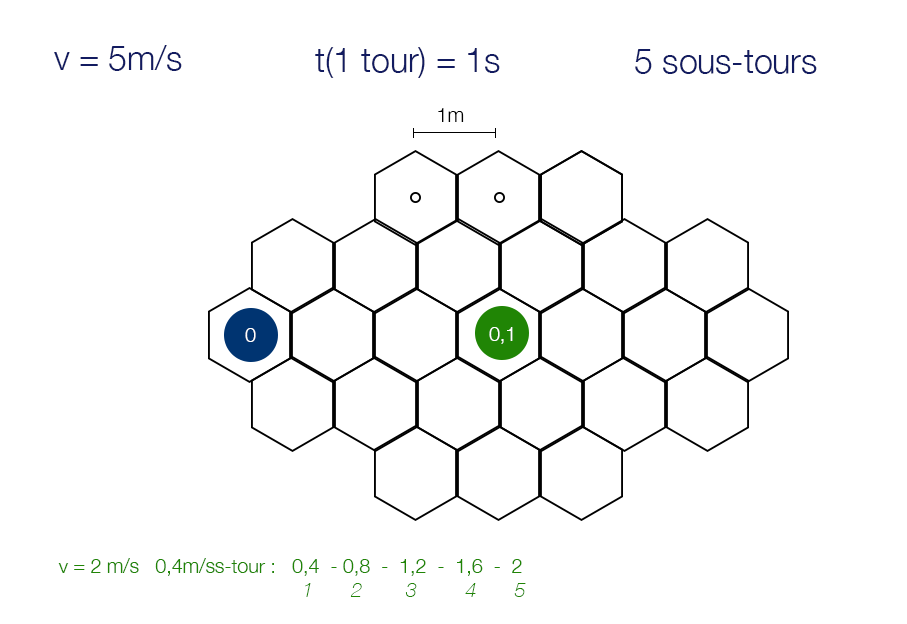
\includegraphics[width=0.3\textwidth]{../TurnModel/TurnModel0.png}
    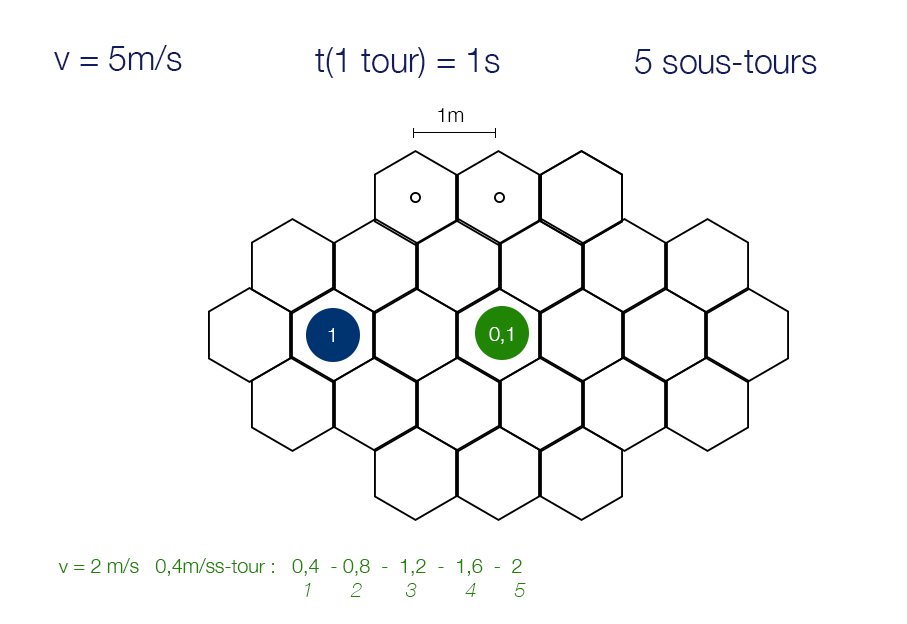
\includegraphics[width=0.3\textwidth]{../TurnModel/TurnModel1.png}
    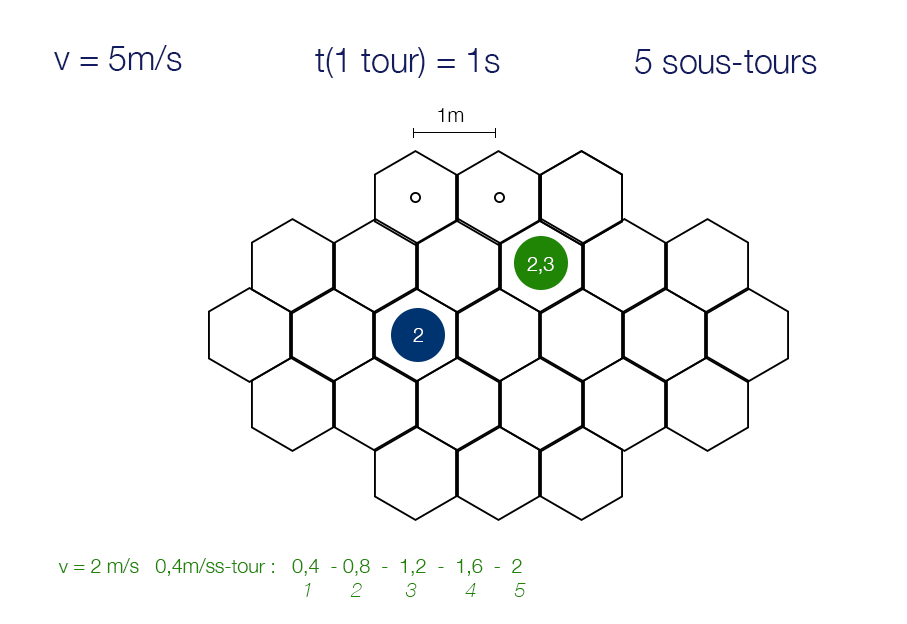
\includegraphics[width=0.3\textwidth]{../TurnModel/TurnModel2.png}
    \\
    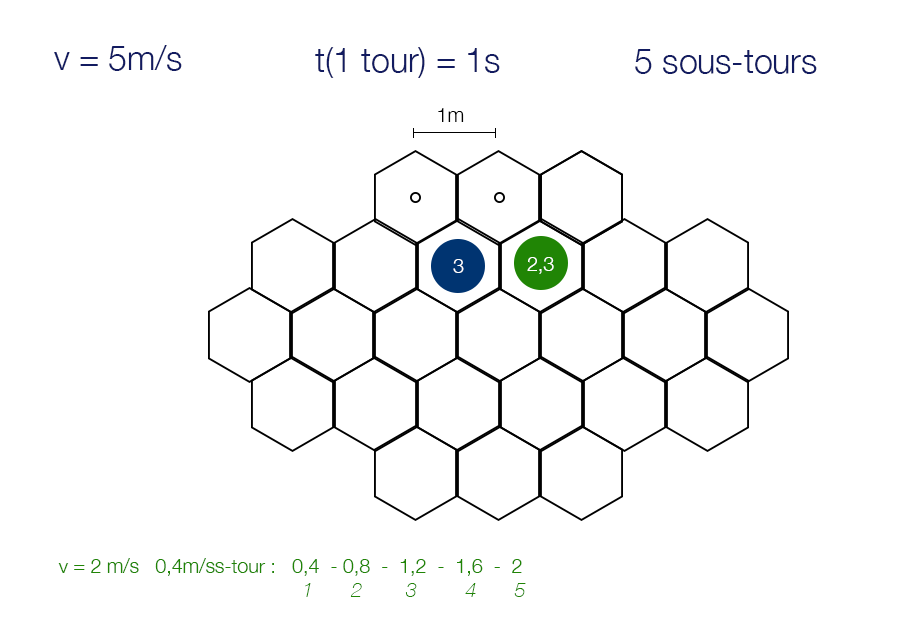
\includegraphics[width=0.3\textwidth]{../TurnModel/TurnModel3.png}
    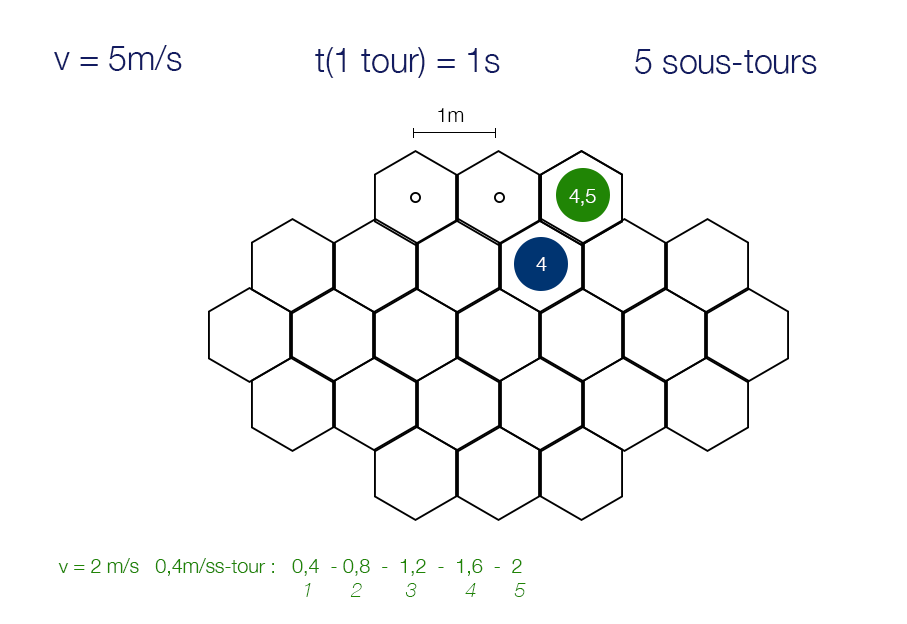
\includegraphics[width=0.3\textwidth]{../TurnModel/TurnModel4.png}
    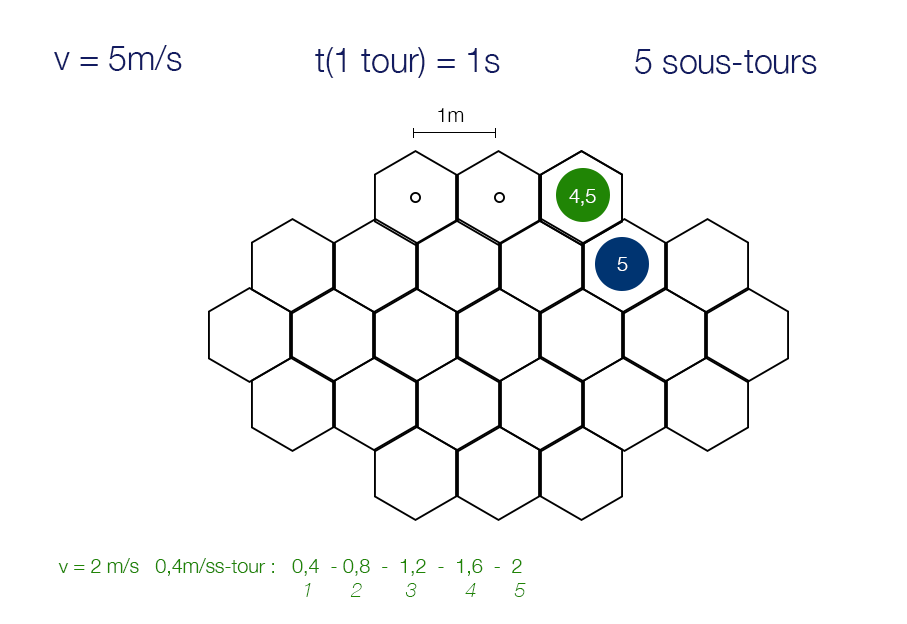
\includegraphics[width=0.3\textwidth]{../TurnModel/TurnModel5.png}
    \caption{\label{fig:TurnModel} Déplacements des joueurs sur le terrain}
\end{figure}

Un tour de jeu est divisé en $n$ intervalles isochroniques, avec $n$ la plus grande vitesse parmis tous les objets déplaçables. La figure \ref{fig:TurnModel} illustre la procédure utilisée. Pour chaque instant, de $t = \frac{1}{n}$ à $t = 1$, pour chaque déplacement à jouer\footnote{Les déplacements sont ordonnés par ordre de réception}, on calcule la position de l'objet déplaçable. Si aucun autre déplaçable ne se trouve à la position calculée, on y place le déplaçable en cours de mouvement. Dans le cas contraire, une collision a lieu.

\subsubsection{Collisions}
Chaque déplaçable a un score de collision, dépendant de ses caractéristiques et d'un jet de dé aléatoire. Lorsqu'une collision a lieu, on demande le score de collision de chacun des déplaçables. Celui ayant le plus grand remporte la case disputée. Plusieurs sous-cas peuvent alors se présenter:

\paragraph{Le premier joueur sur la case gagne}
Le second prétendant à cette position voit son mouvement arrêté. Il es placé sur la dernière case qu'il a atteint et son déplacement est supprimé de la case

\paragraph{Le second arrivant gagne}
Le premier joueur est placé sur une case libre adjacente, son mouvement est supprimé, et le second joueur lui vole la position.

\paragraph{Un des deux déplaçable est attrapable par l'autre}
Le joueur attrape l'autre déplaçable.


\appendix

\chapter{À propos de la librairie graphique}
Nous avons choisi d'utiliser la SFML (simple and fast multimedia library) dans l'optique de notre projet. 

Cette librairie open-source a été codée en C++ spécialement pour le développement de jeux 2D, et permet l'utilisation de la programmation orientée objet, s'accordant donc avec l'optique de ce travail : apprendre le développement d'applications à des étudiants universitaires. De plus, le site web de la librairie\footnote{http://www.sfml-dev.org/} regorge de documentation et tutoriels.

Une alternative envisagée était SDL, fer de lance du développement de jeux 2D, mais l'utilisation intensive d'OpenGL par la SFML rend celle-ci souvent plus rapide dans son exécution\footnote{http://en.sfml-dev.org/forums/index.php?topic=43.0}.

Enfin, pour ne rien gâcher, la SFML possède une communauté très active, et tout particulièrement la communauté francophone, le développeur étant lui-même Français.

\chapter{Diagramme de classes général}
\begin{figure}[ht]
  \centering
  \includegraphics[angle=90,width=0.4\textwidth]{figures/general-class.eps}
  \caption{\label{fig:Class:General} Classes: diagramme général}
\end{figure}

\printindex
\listoffigures

\end{document}
